%\documentclass[handout]{beamer}
\documentclass[ignorenonframetext]{beamer}
\usepackage{textpos}
\usepackage{graphicx}
\usepackage{pgf}
\usepackage{caption}
\usepackage{multimedia}
\usepackage{gensymb}
\usepackage{amsmath, mathrsfs}

\captionsetup[figure]{labelformat=empty}% redefines the caption setup of the figures environment in the beamer class.

\usetheme{Boadilla}
\usefonttheme{serif}
% \mode<presentation>
% {
%  \usefonttheme{serif}
% % \useoutertheme{sidebar}
% %   \logo{
\includegraphics[height=1cm]{elec_logo.pdf}}
% }

\title[TART]{The Transient Array Radio Telescope (TART) Overview}

\author[Molteno]{Tim Molteno}

\institute[Otago]
{
  Department of Physics\\
  University of Otago \\
  Dunedin, New Zealand.\\
  tim@elec.ac.nz\\
  \vspace{2cm}
  
\includegraphics[width=0.7\linewidth]{fig/elec_header_font.pdf}
}

% \titlegraphic{
\includegraphics[width=2cm]{fig/elec_logo.pdf}\hspace*{4.75cm}~%
%    
\includegraphics[width=2cm]{fig/elec_logo.pdf}
% }

\logo{\pgfputat{\pgfxy(-0.72,7.7)}{\pgfbox[center,base]{
\includegraphics[width=1cm]{fig/elec_logo.pdf}}}} 

\date[TART-Workshop] % (optional, should be abbreviation of conference name)
{}

% \addtobeamertemplate{headline}{}{%
% \begin{textblock*}{100mm}(0.87\textwidth,2mm)
% 
\includegraphics[height=1.5cm]{elec_logo.pdf}
% \end{textblock*}}

\begin{document}



\begin{frame}
  \titlepage
\end{frame}

% \begin{frame}{Abstract}
%  I will introduce the Transient Array Radio Telescope. Developed here in the Department of Physics at Otago University, this is the worlds smallest (and cheapest) aperture synthesis radio telescope -- that is a telescope that creates images of the radio sky. It is now being used by astronomers working on the Square Kilometer Array, the worlds largest radio telescope -- as an instrument that can be used to both develop new algorithms for radio astronomy and also to teach students about how radio telescopes work. I will describe the instrument and how it works, as well as giving an overview of the upcoming projects involving this telescope in Africa.
% \end{frame}

\begin{frame}
  \tableofcontents
  % You might wish to add the option [pausesections]
\end{frame}

\section{TART: Prehistory}

\begin{frame}{TART: Single-Dish Engineering Prototype}
   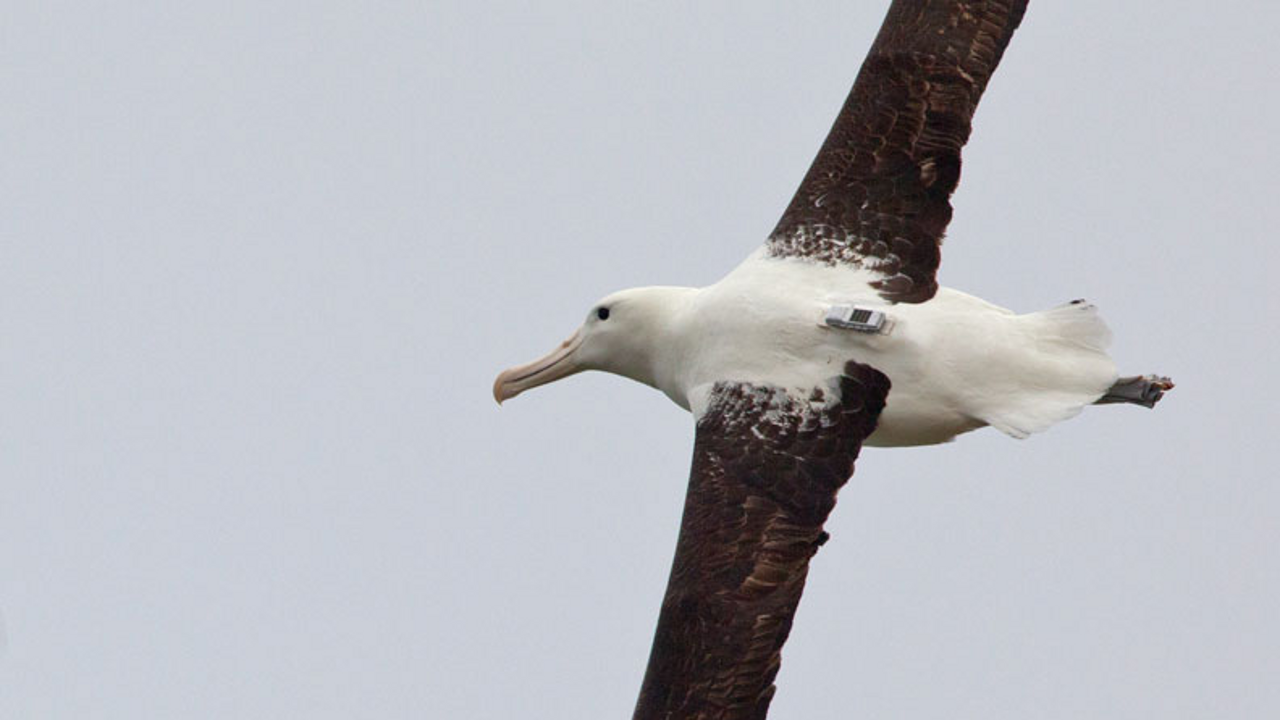
\includegraphics[width=\linewidth]{fig/albatross_frame.png}
\end{frame}

\begin{frame}{TART: Evaluation}
   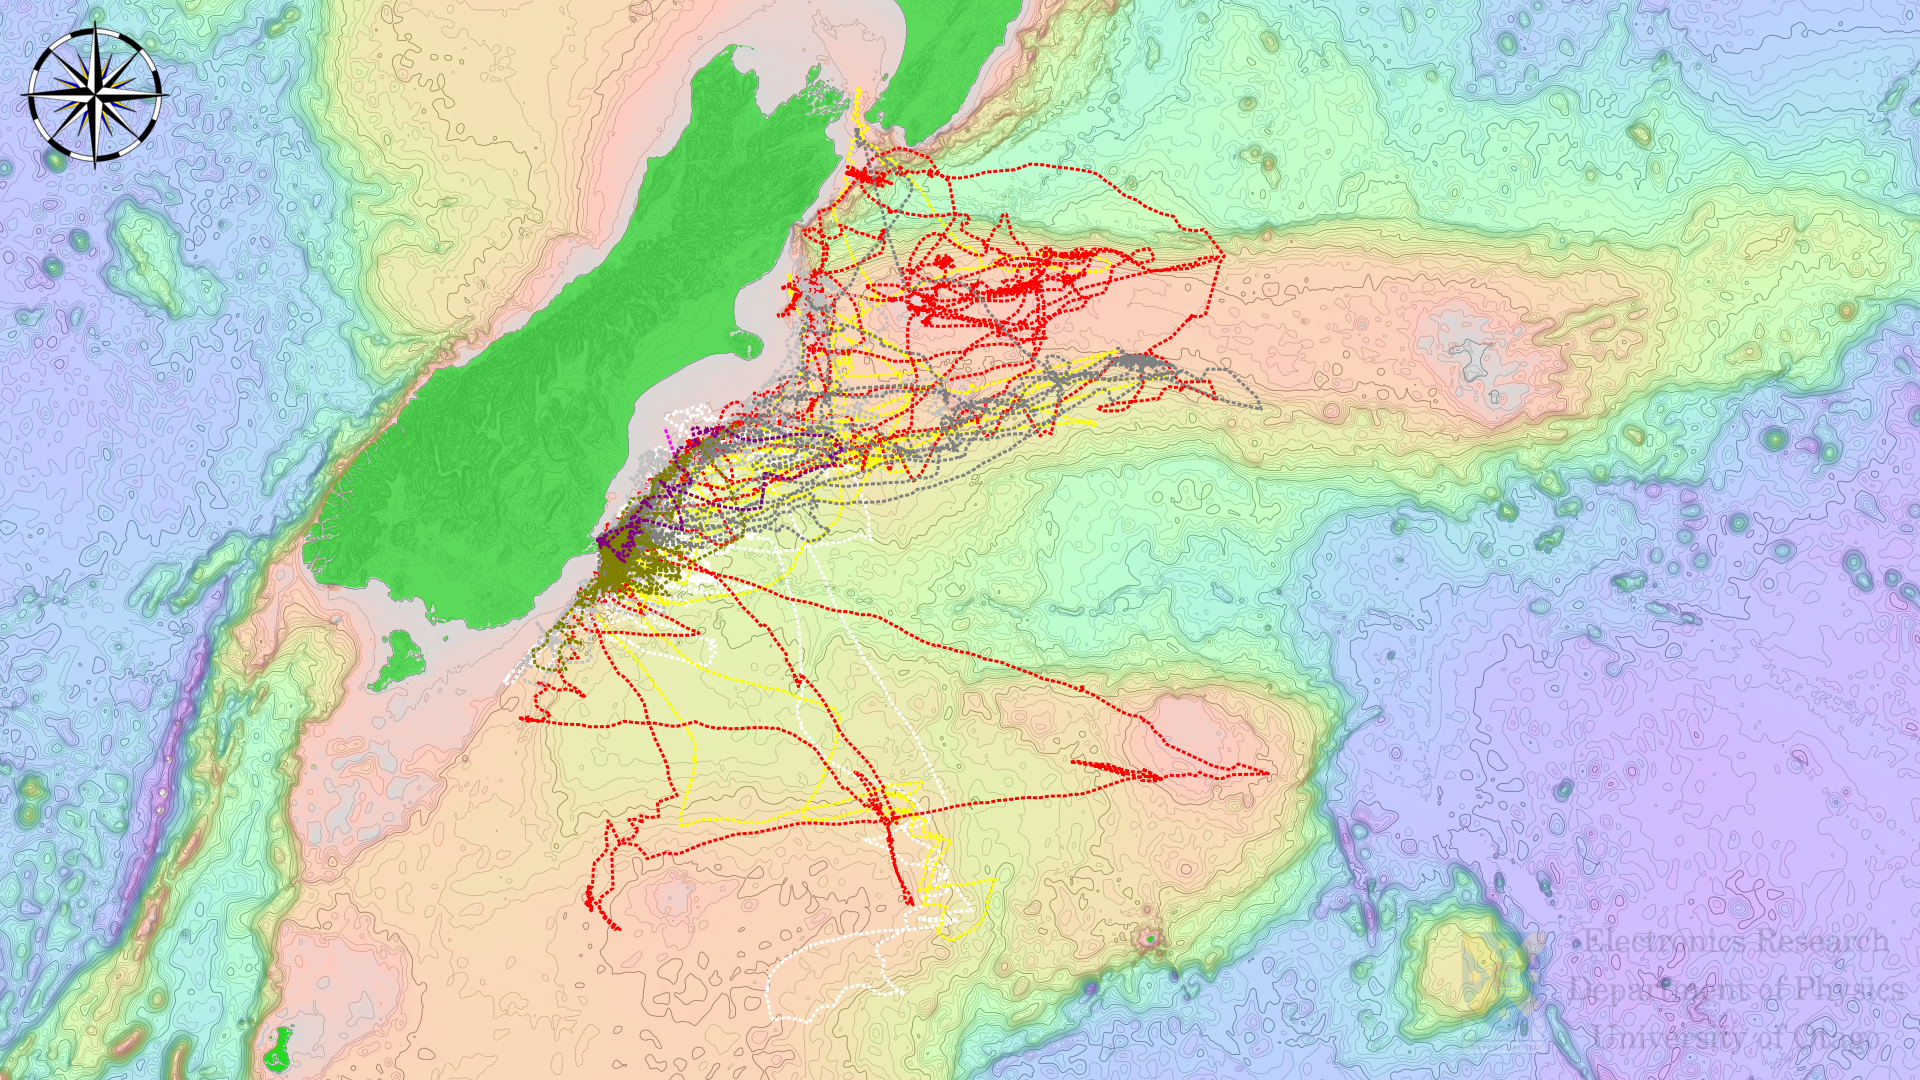
\includegraphics[width=\linewidth]{fig/project_map_14.png}
\end{frame}


%  \begin{columns}
%   \begin{column}{0.5\linewidth}
%   \begin{center}
%     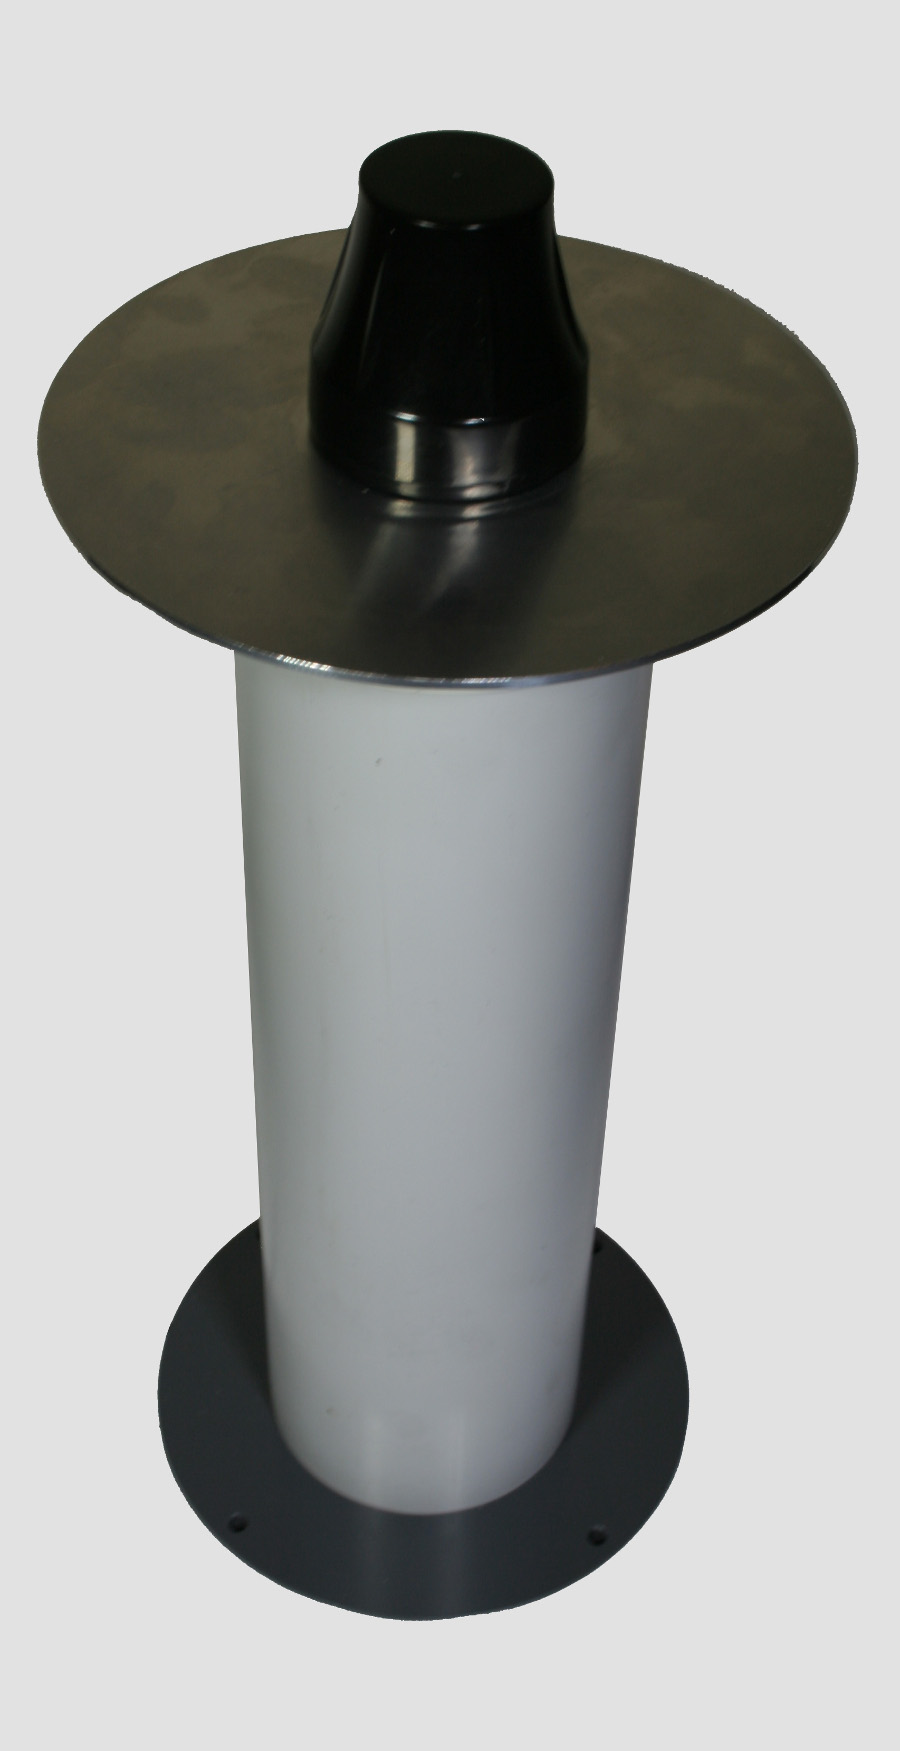
\includegraphics[height=0.4\textheight]{fig/antenna.jpg}
%   \end{center}
%   \end{column}
%   \begin{column}{0.5\linewidth}
%    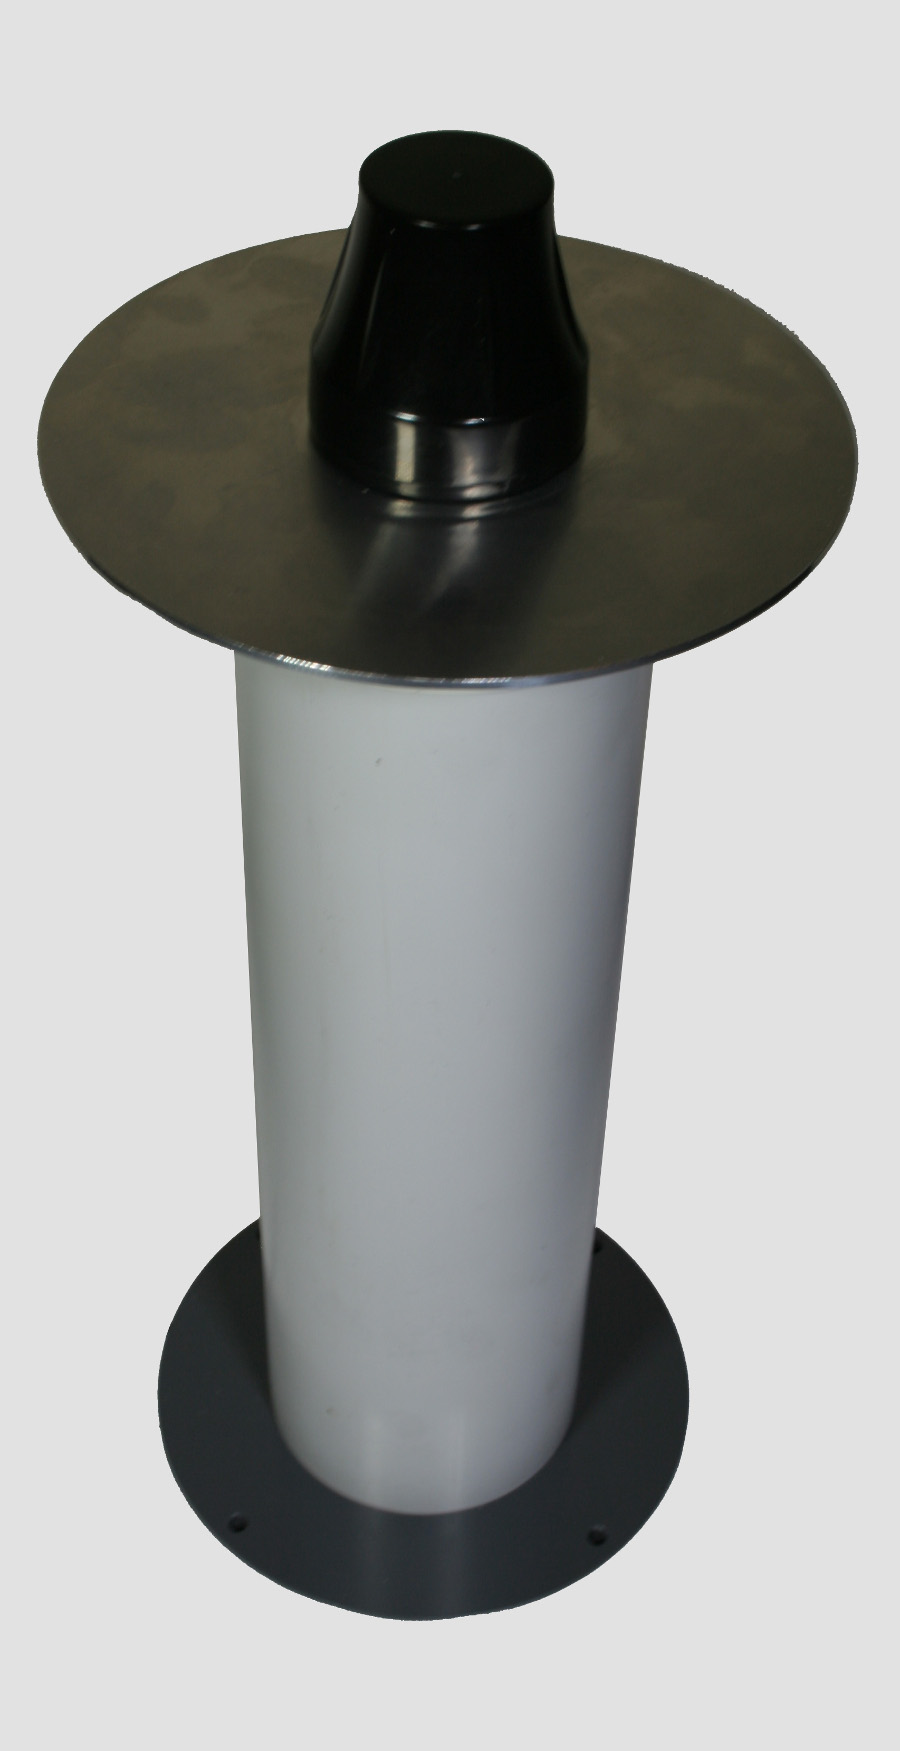
\includegraphics[width=\textwidth]{fig/antenna.jpg}
%   \end{column}
%  \end{columns}
% 

% \section{Aperture synthesis Radio Telescopes}

% 
% \begin{center}
%   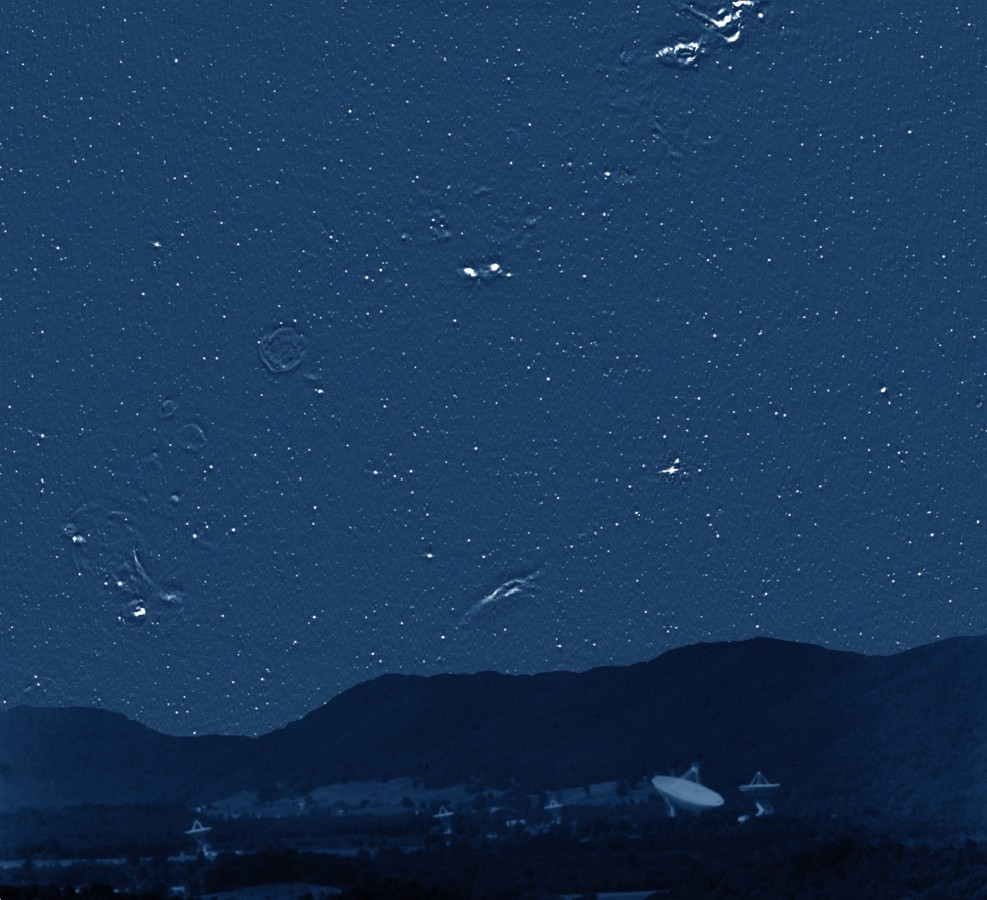
\includegraphics[width=0.45\linewidth]{fig/RadioNightSky_med.jpg}
%   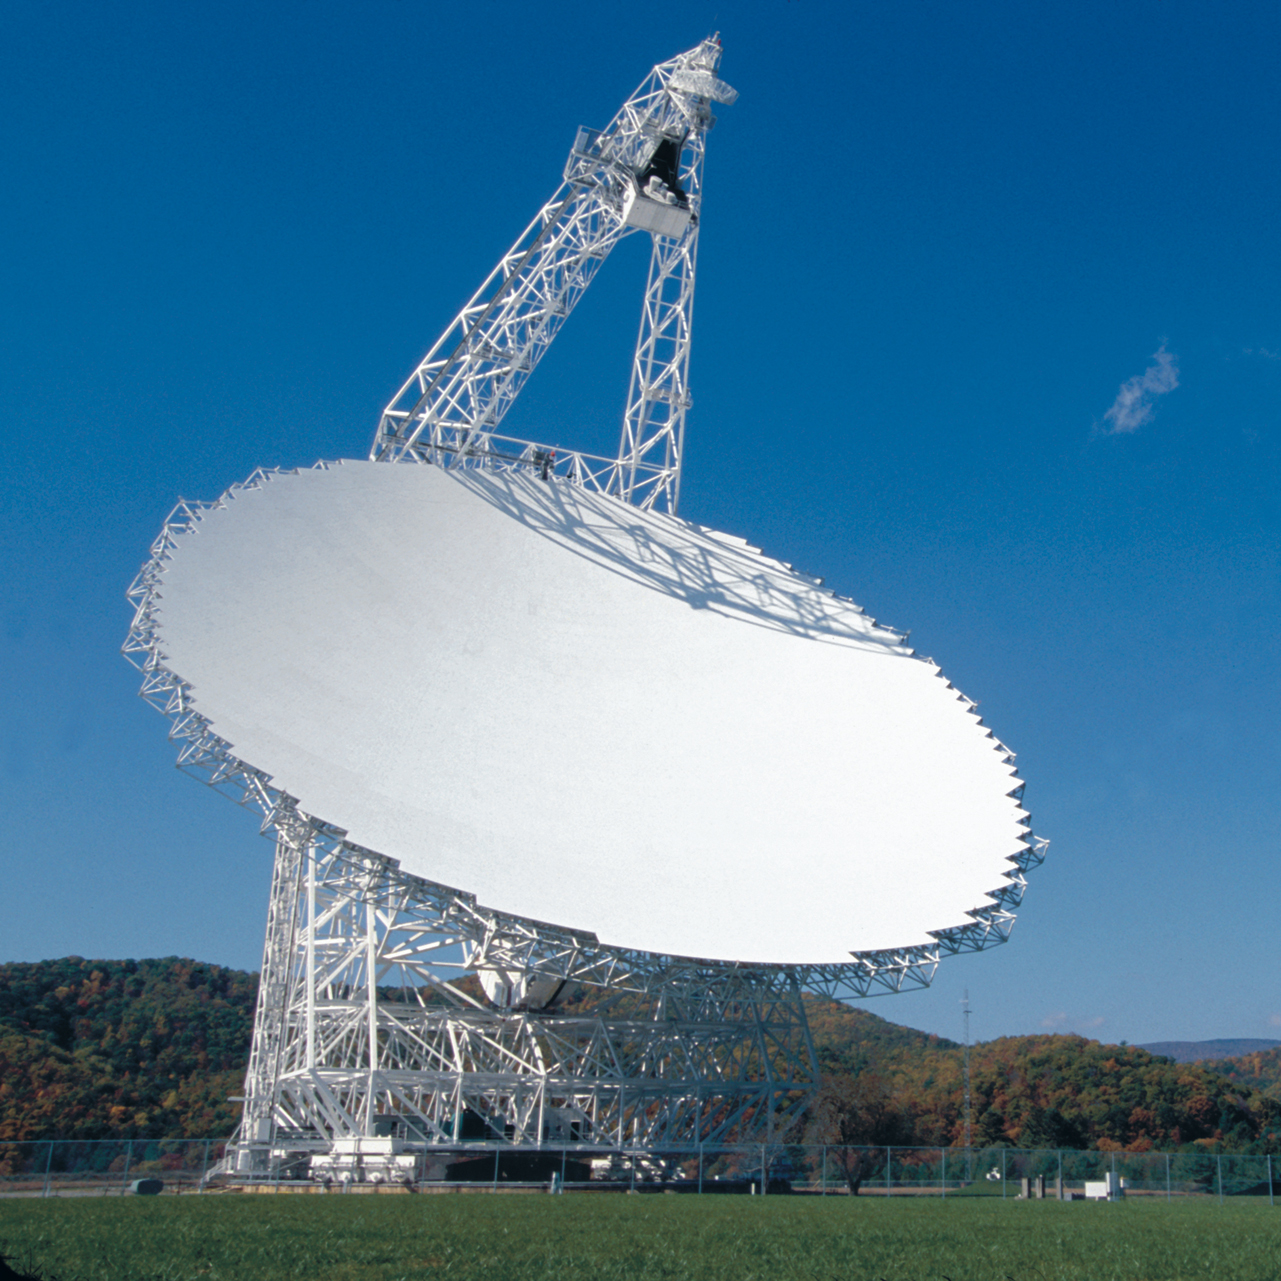
\includegraphics[width=0.45\linewidth]{fig/green_bank.jpg}
% \end{center}
% \end{frame}

% \begin{frame}{Aperture synthesis Radio Telescopes}
% \begin{center}
%   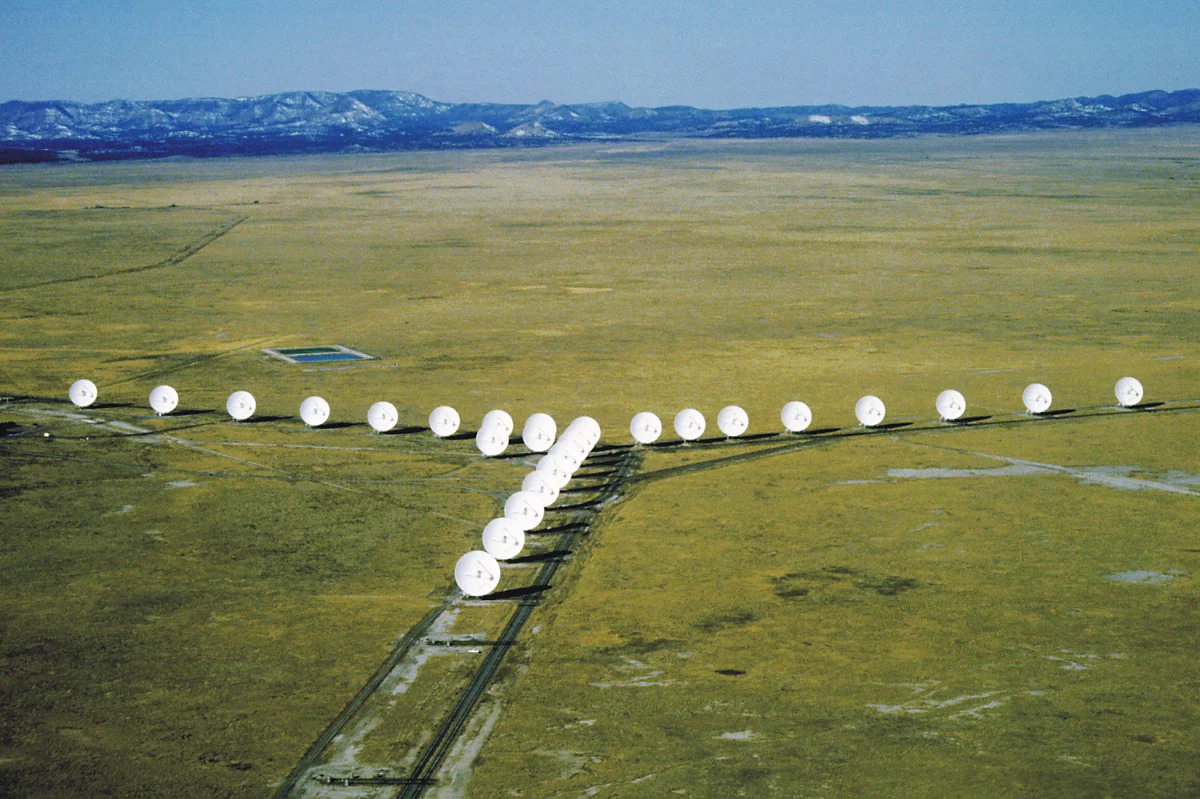
\includegraphics[width=\linewidth]{fig/vla_large.jpg}
% \end{center}
% \end{frame}

\section{MeerKAT: The world's biggest radio telescope}

\frame{\tableofcontents[currentsection]}

\begin{frame}{MeerKAT: Africa centre of radio astronomy}
\begin{center}
  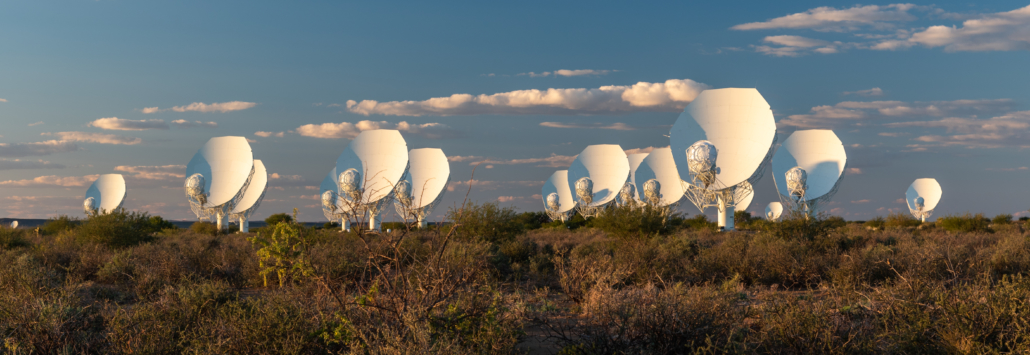
\includegraphics[width=\linewidth]{fig/2018-MeerKAT-5-1030x355.jpg}
\end{center}
\begin{itemize}
 \item 13.5 meter antennas. 143 $m^2$
 \item 64 of them!
 \item Frequency Range: 900 MHz - 1670 MHz
 \item SKA pathfinder
\end{itemize}

\end{frame}


\begin{frame}{MeerKAT: The Centre of our Galaxy}
 \begin{center}
  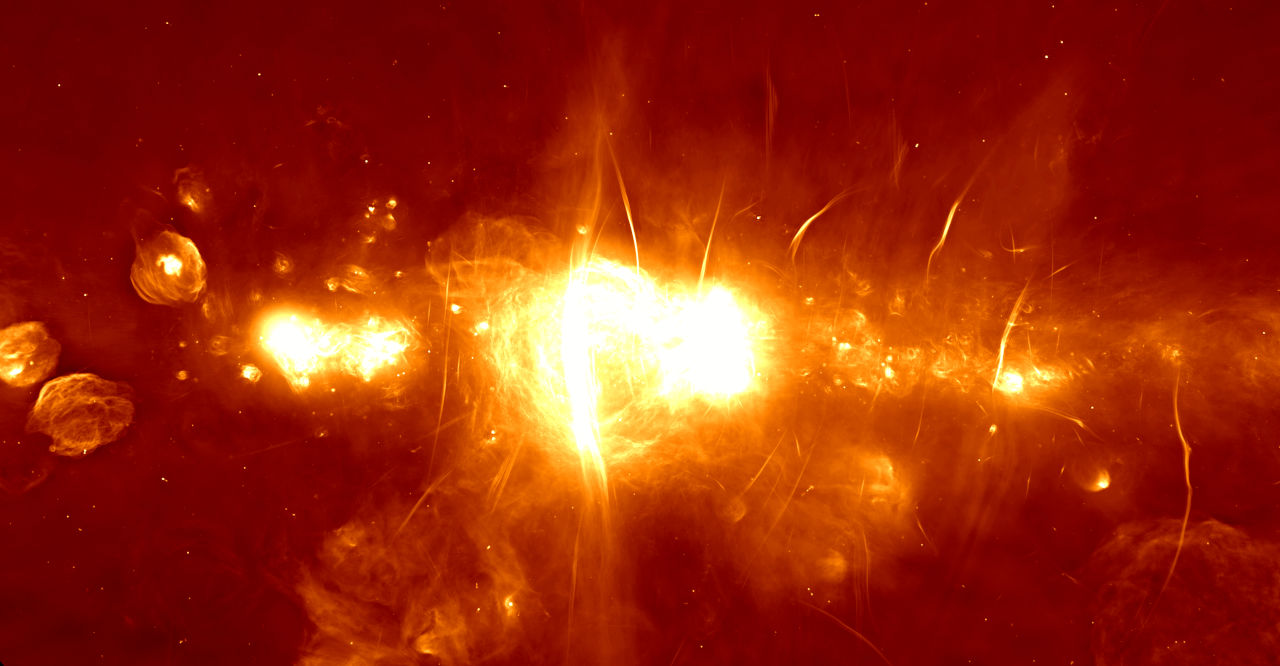
\includegraphics[width=\linewidth]{fig/MeerKAT_GalacticCentre_image.jpeg}
 \end{center}

\end{frame}


\begin{frame}{MeerKAT: It's very precious}
MeerKAT is currently the worlds biggest radio telescope
\begin{itemize}
\item SKA pathfinder
\item Total cost: billions
\item Running cost: millions
\item A long queue of eager astronomers...
\end{itemize}

\includegraphics[width=0.32\linewidth]{fig/ska-logo-color.pdf}

\includegraphics[width=0.32\linewidth]{fig/NRF_SARAO_sm1.png}
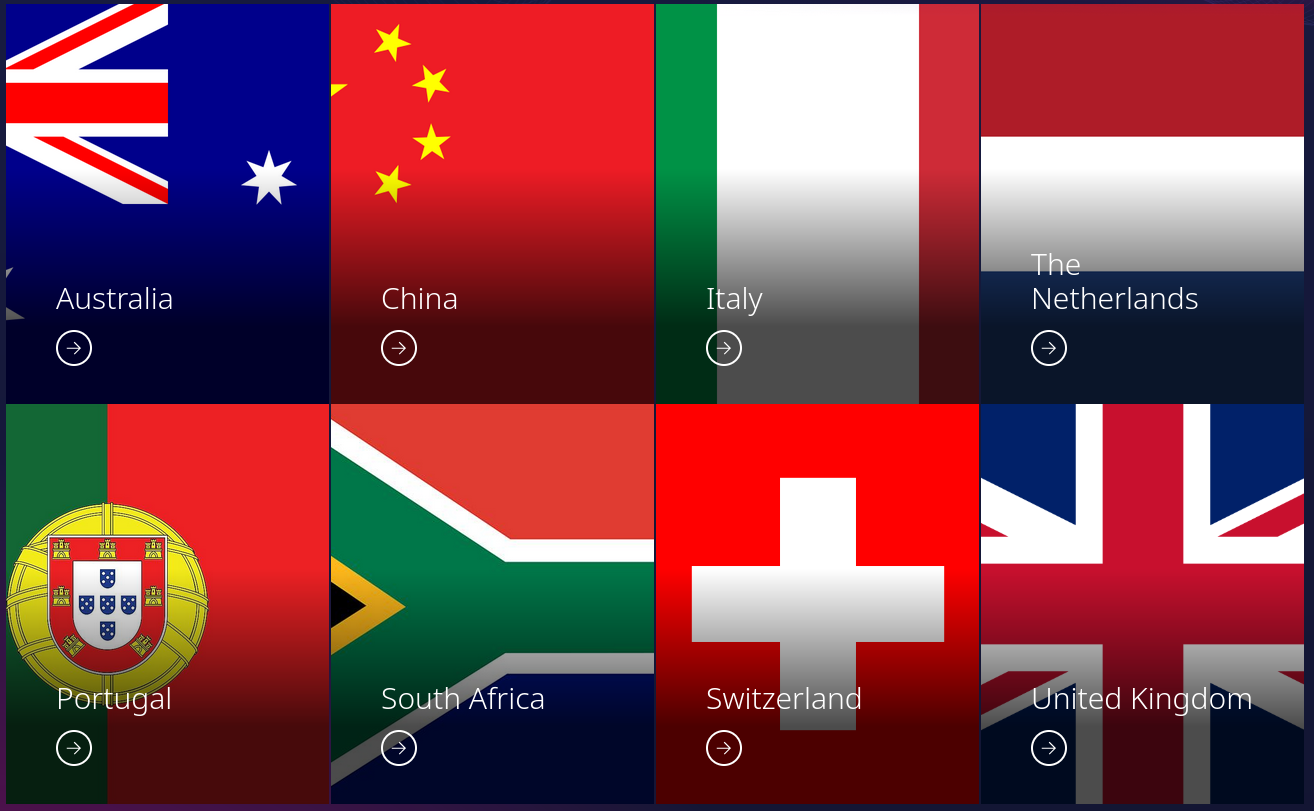
\includegraphics[width=0.32\linewidth]{fig/ska-partners.png}
\end{frame}

\section{TART: The worlds smallest radio telescope}

\frame{\tableofcontents[currentsection]}

% 
% \begin{frame}
%   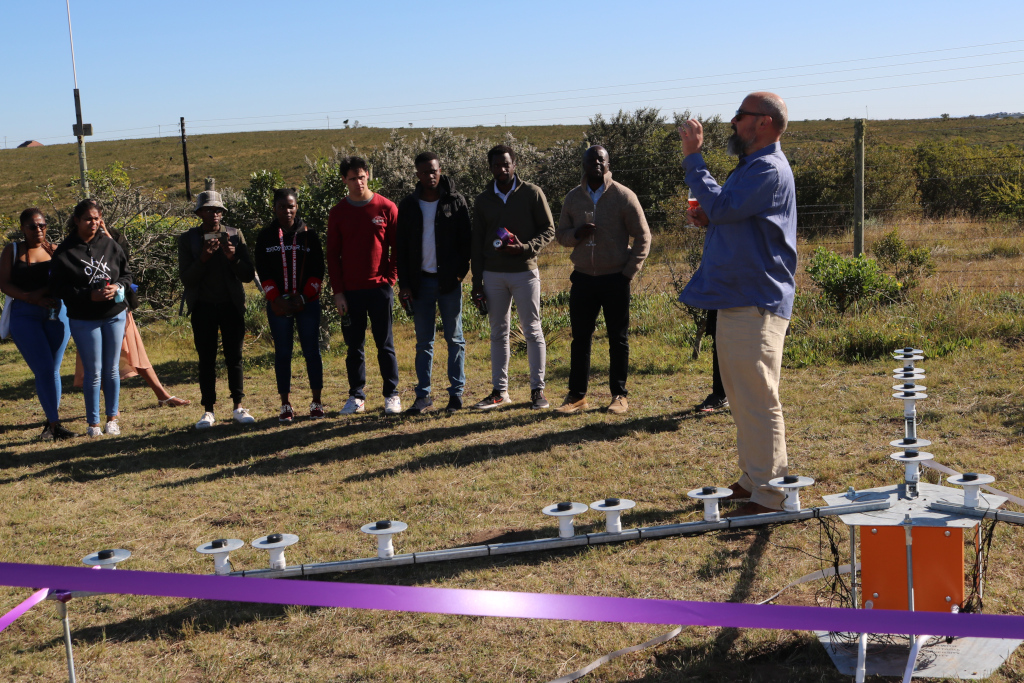
\includegraphics[width=\linewidth]{fig/rhodes_opening.jpg}
% \end{frame}
% 
% \begin{frame}
%   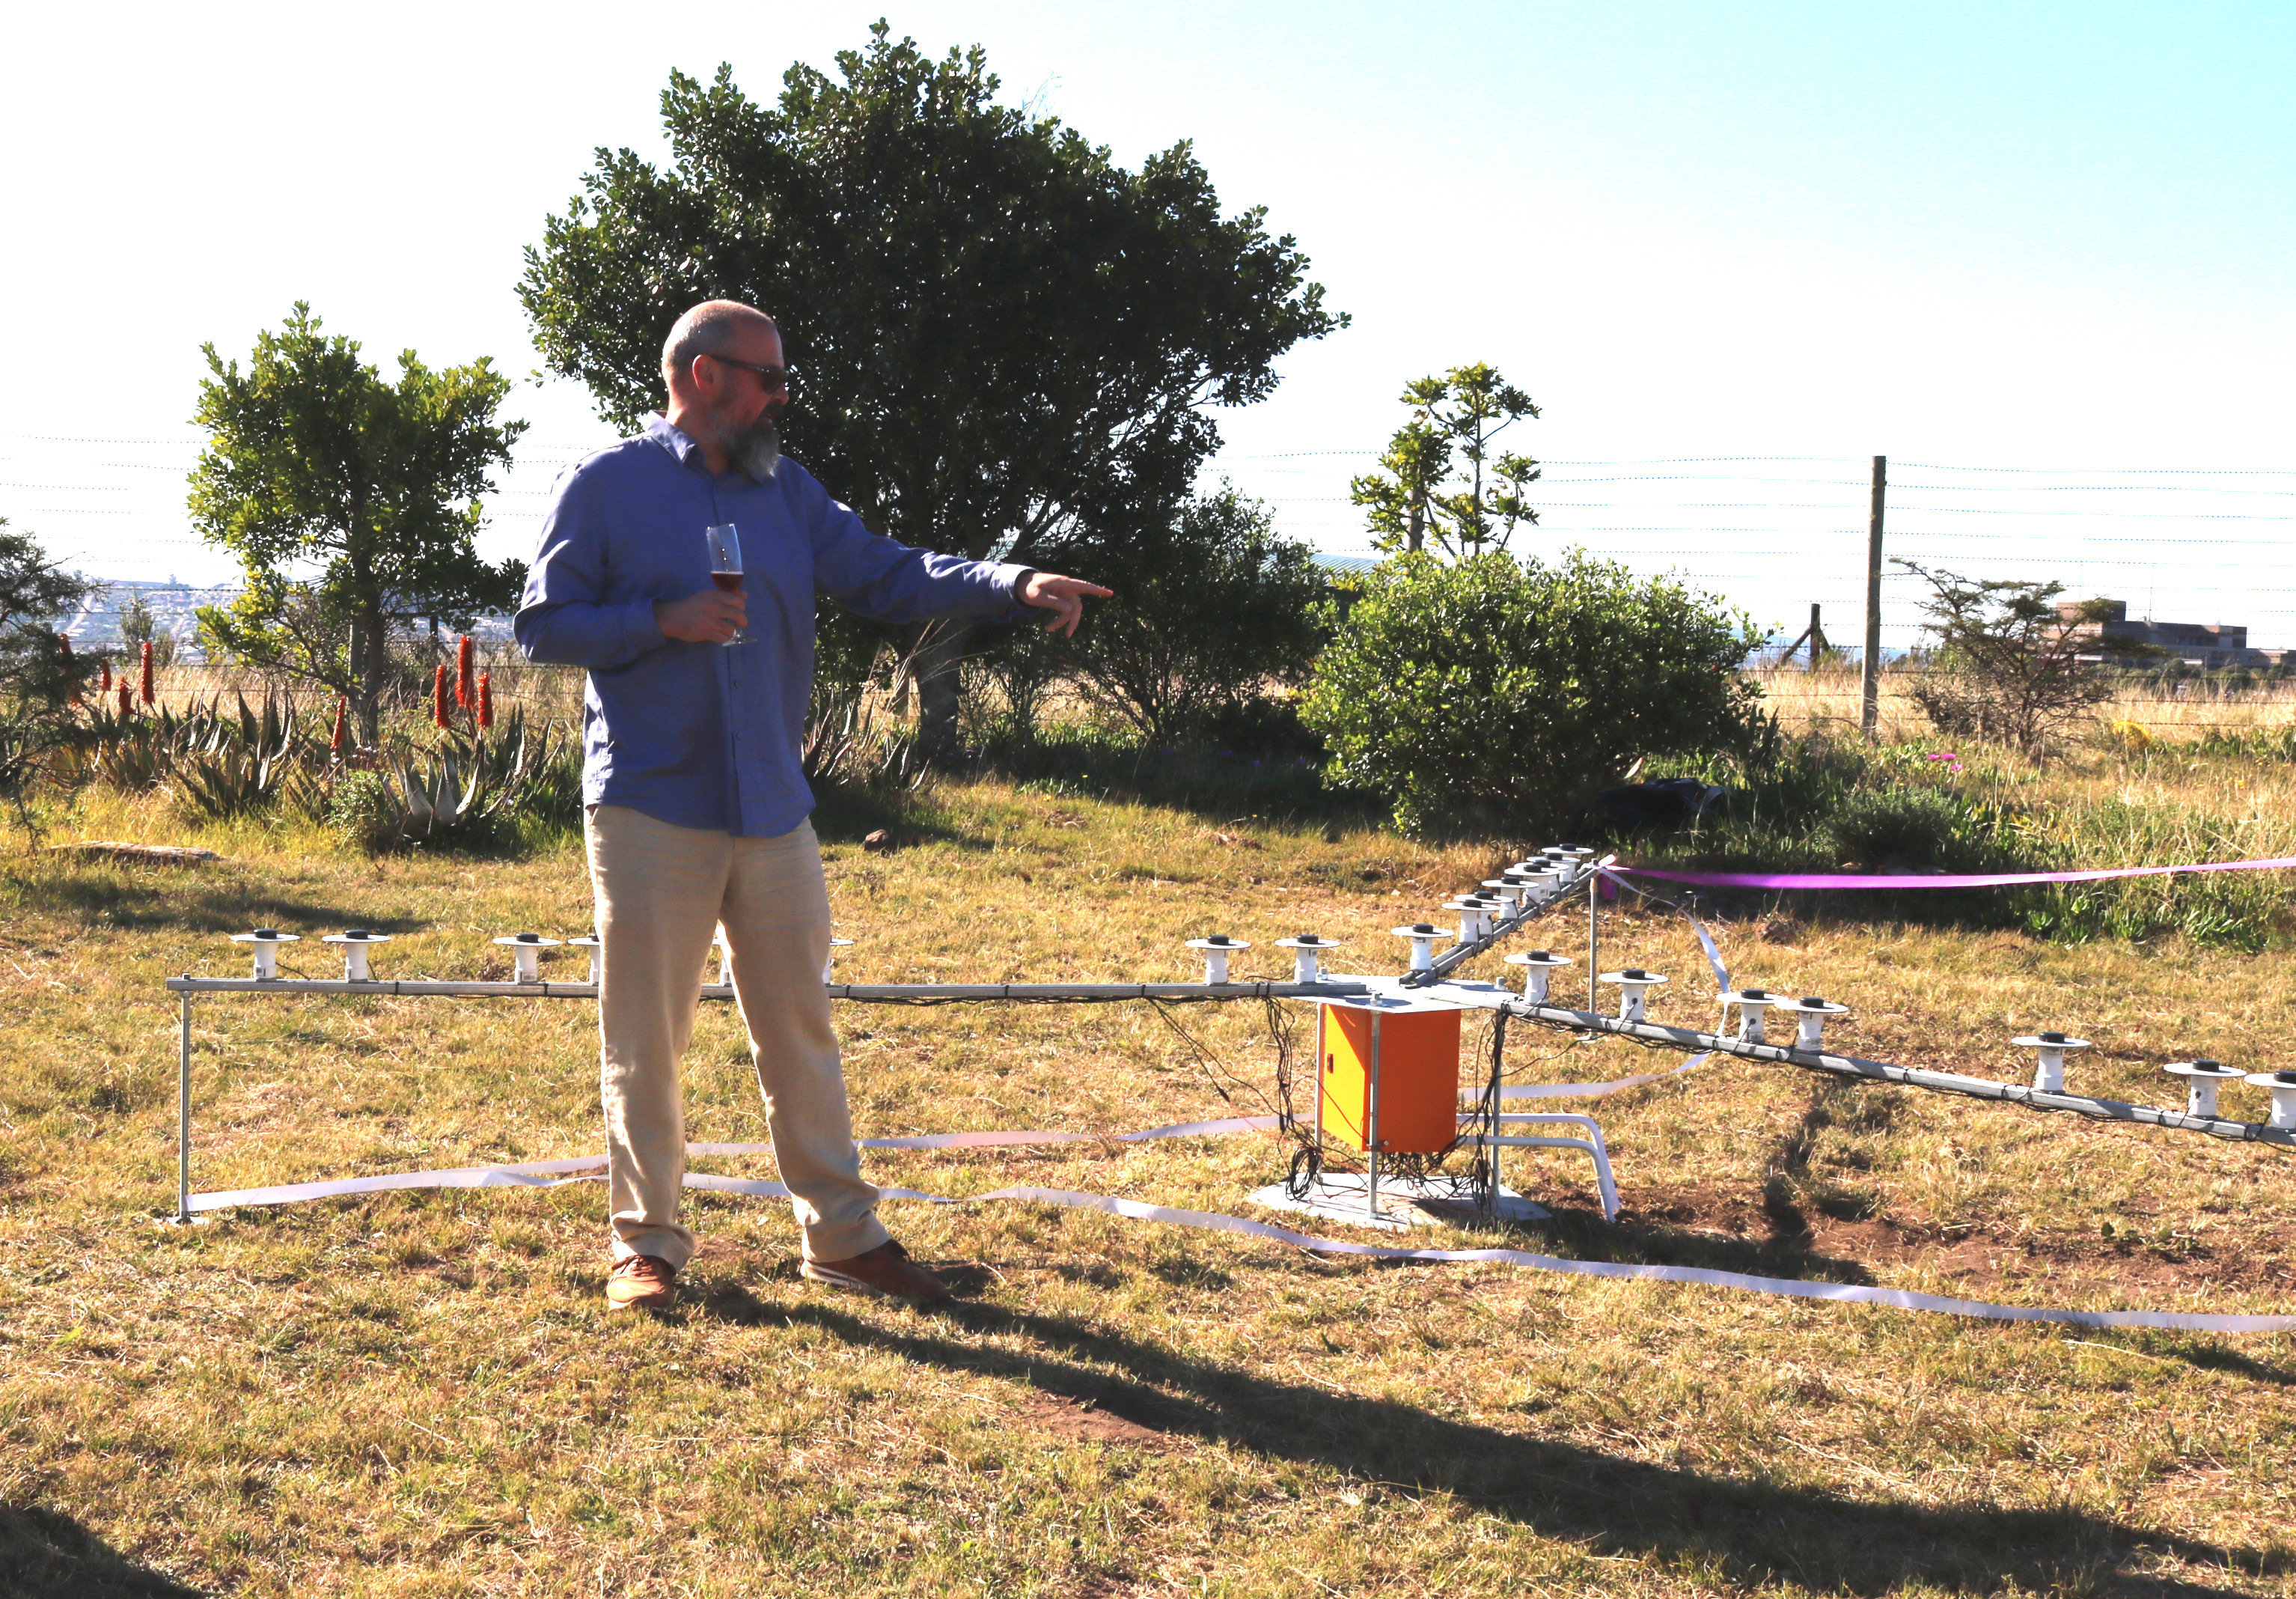
\includegraphics[width=\linewidth]{fig/rhodes_photo_array.jpg}
%   \includegraphics[height=0.4\textheight]{fig/rhodes_photo_elec.jpg}
% \end{frame}



\begin{frame}{TART-2: Overview}
 \begin{columns}
  \begin{column}{0.4\linewidth}
   \begin{itemize}
    \item Array radio telescope
    \item 24 receivers
    \item Real-time correlation in FPGA
    \item Open-Source Design
    \item Cost: \$1000 Euro
   \end{itemize}
   \begin{center}
  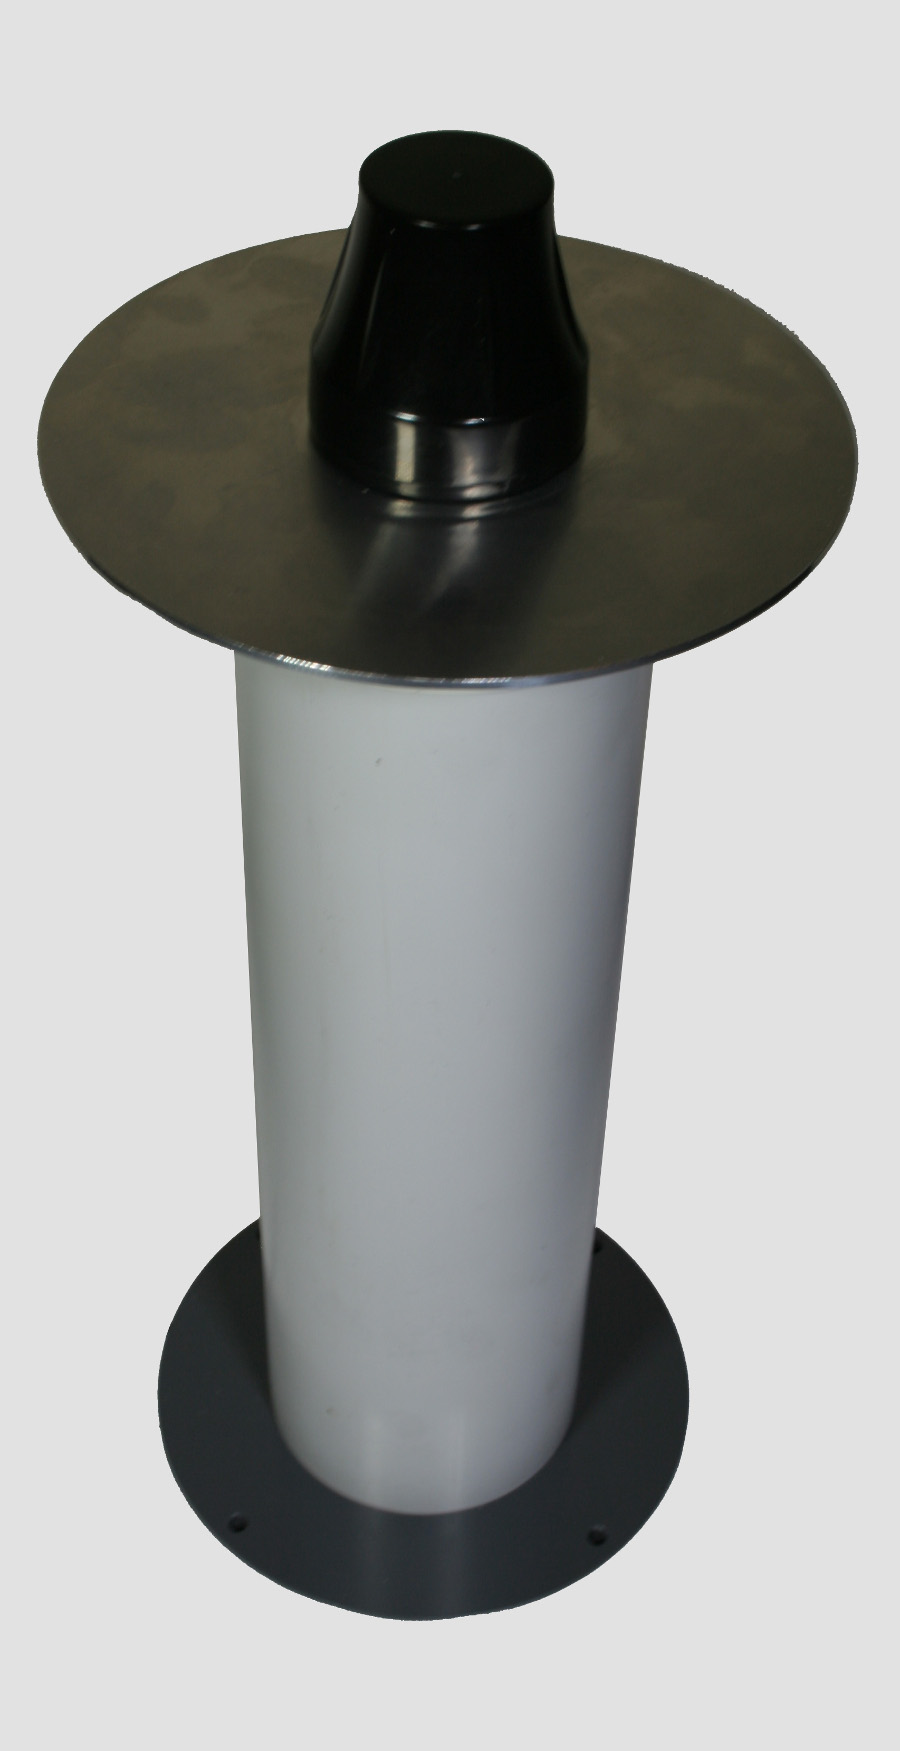
\includegraphics[height=0.4\textheight]{fig/antenna.jpg}
  \end{center}
  \end{column}
  \begin{column}{0.6\linewidth}
   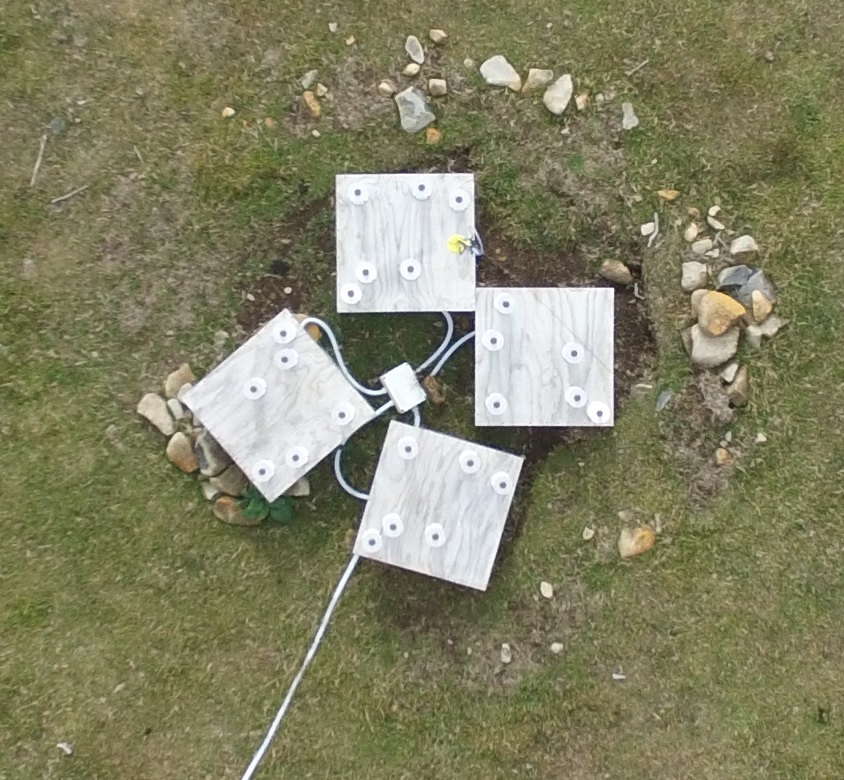
\includegraphics[width=\textwidth]{../../../papers/2019_iceaa/top_view.jpg}
  \end{column}
 \end{columns}
\end{frame}


\begin{frame}{TART-2: Installation at Rhodes}
\begin{center}
  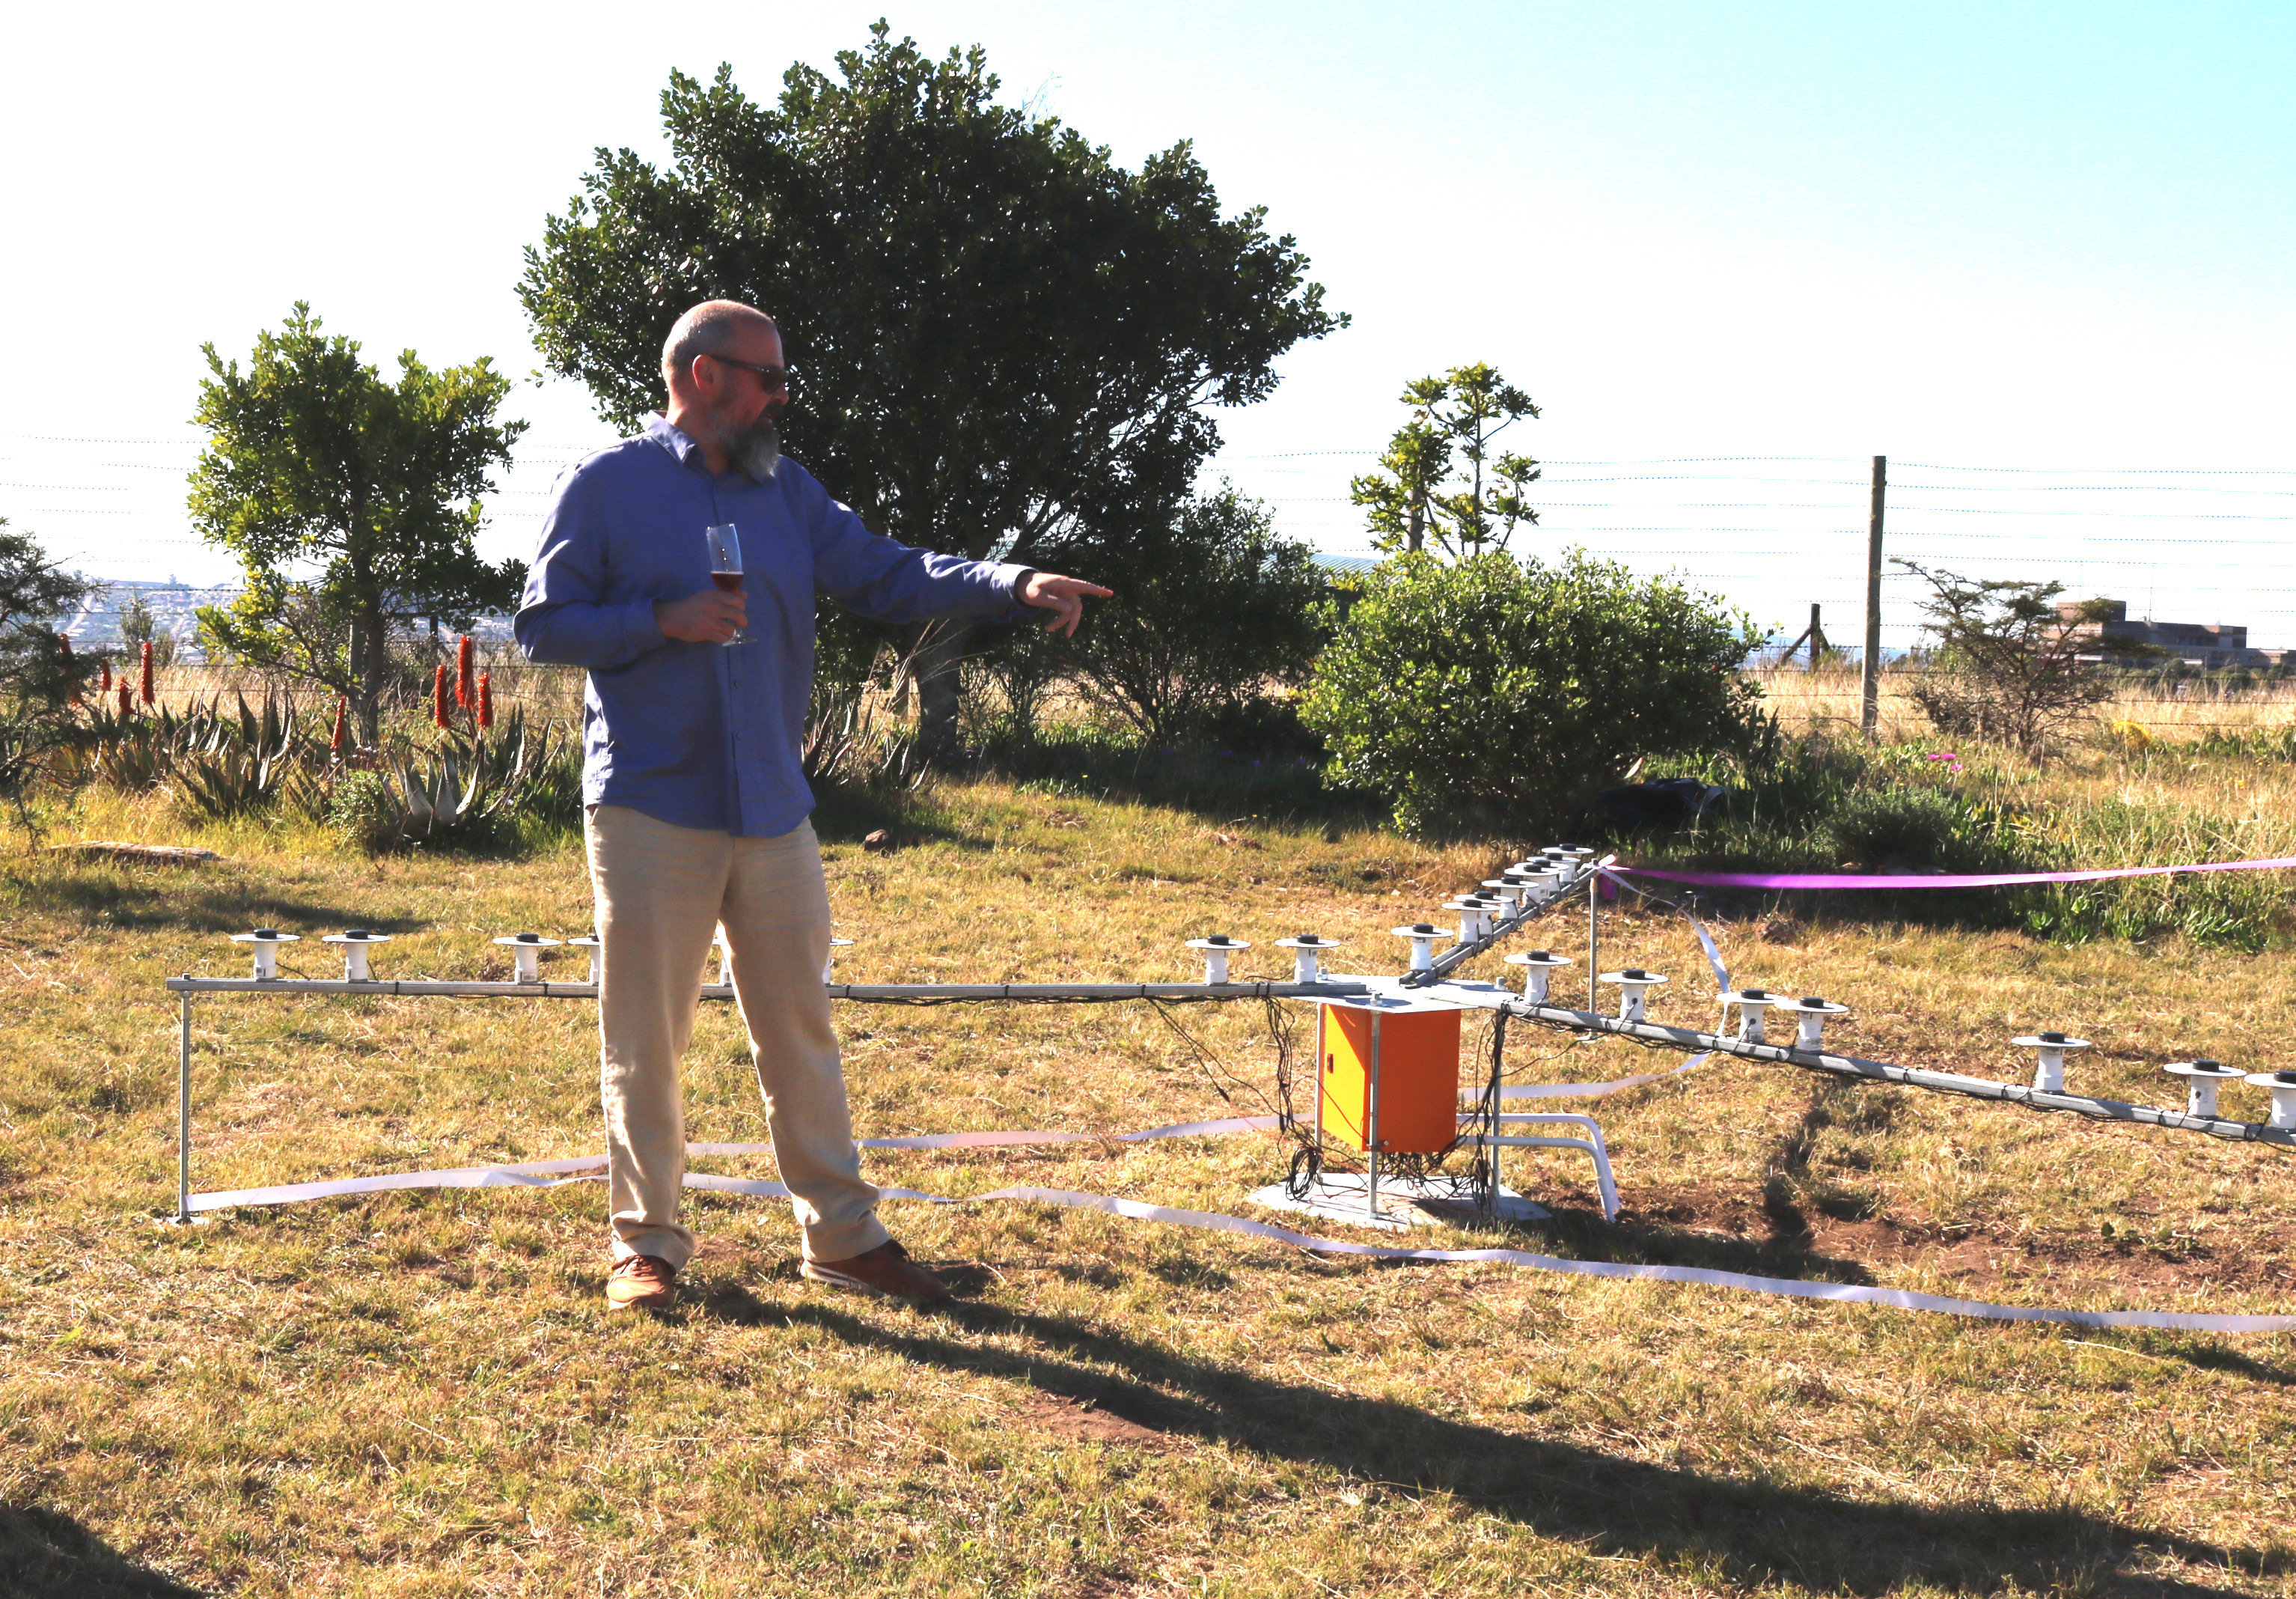
\includegraphics[width=0.9\linewidth]{fig/rhodes_photo_array.jpg}
\end{center}
\begin{itemize}
 \item 0.025 meter antennas. 0.0005 $m^2$.
 \item Frequency Range: 1575.42 MHz ($\pm 4$)
 \item Dunedin, NZ, Rhodes \& Stellenbosch South Africa.
\end{itemize}
\end{frame}

\begin{frame}
\vspace{1cm}
  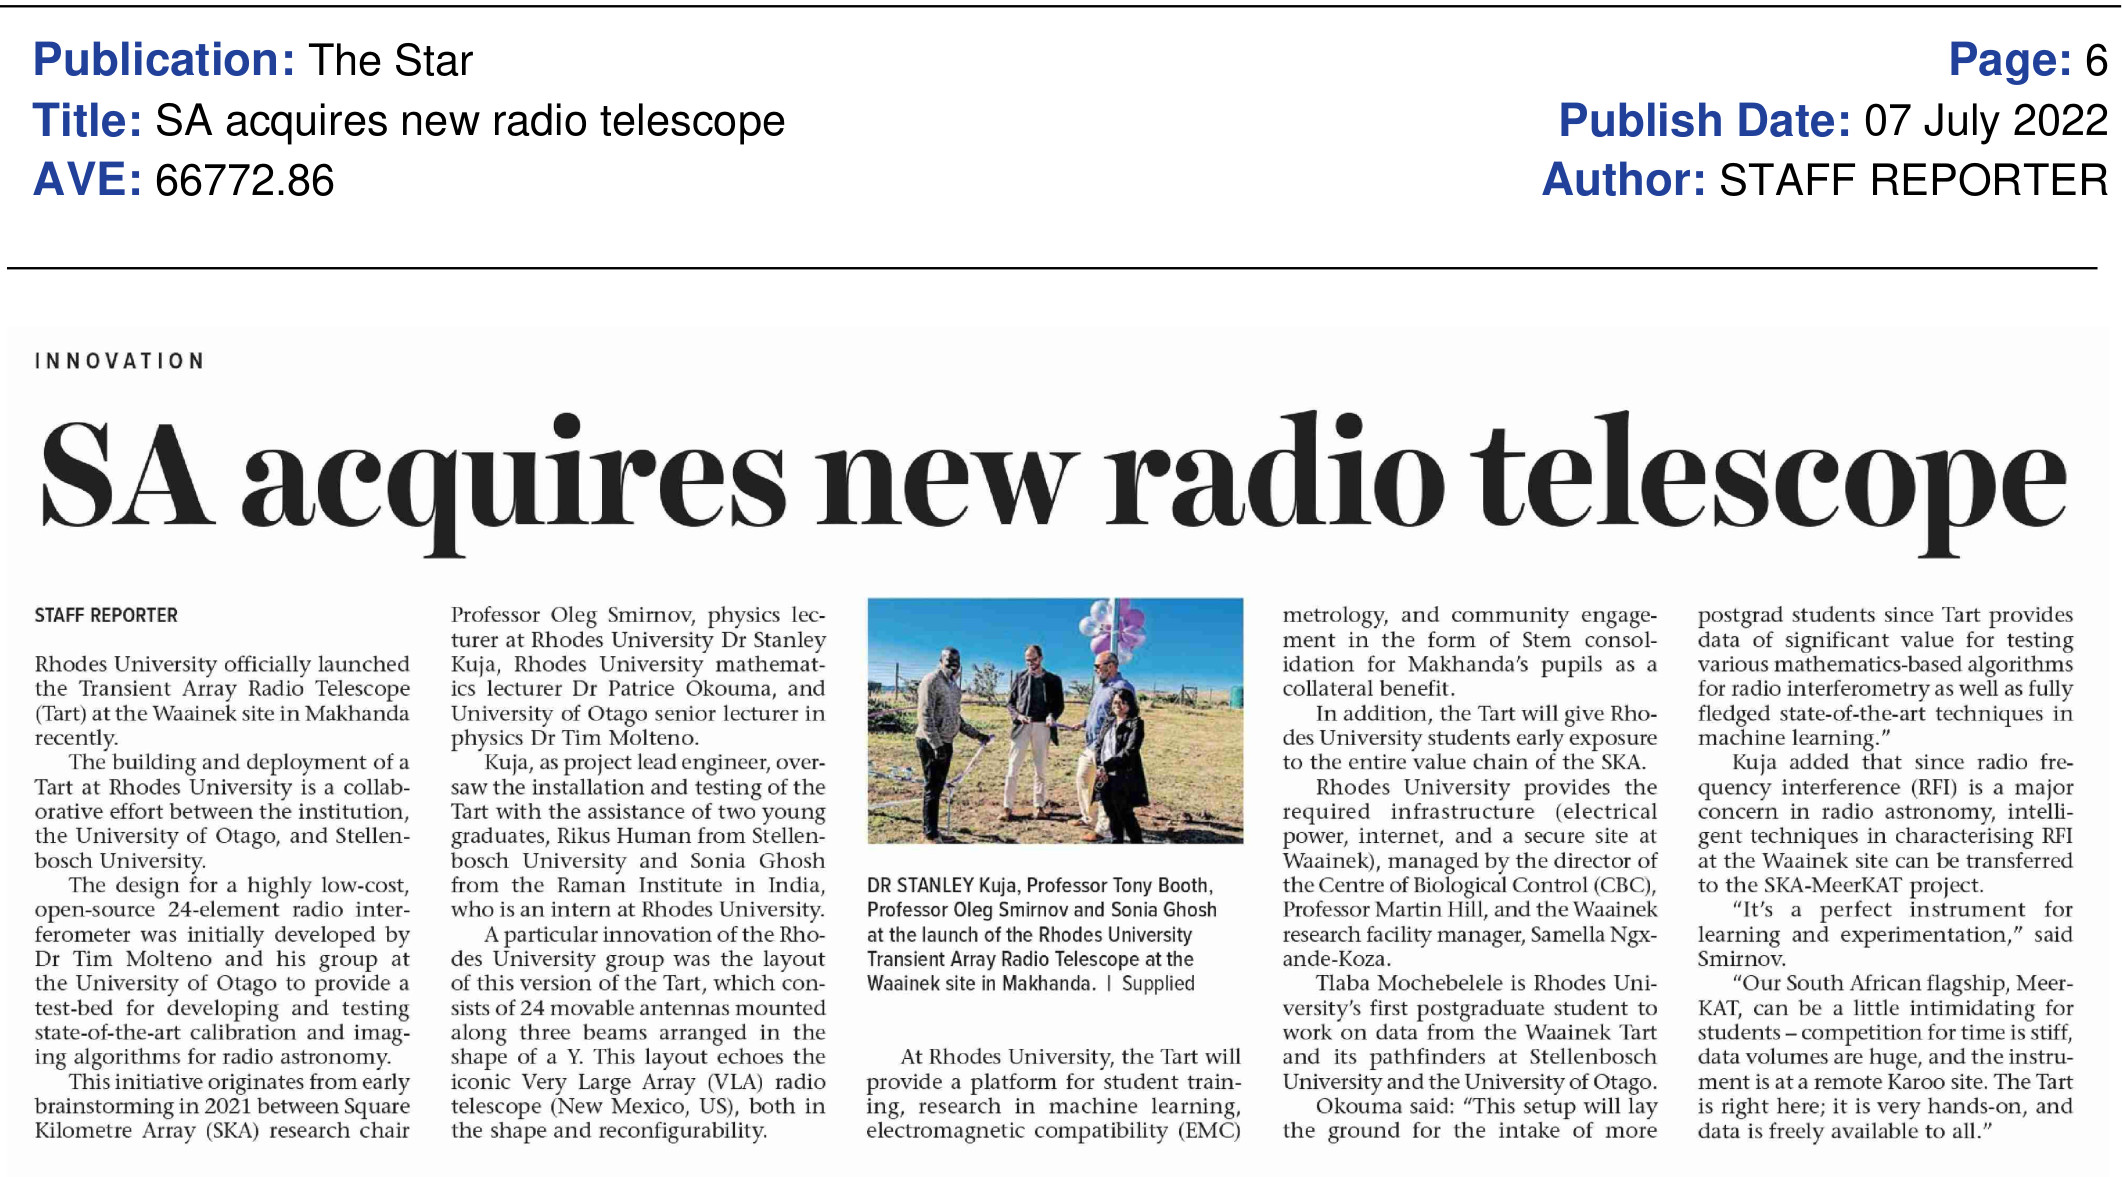
\includegraphics[width=\linewidth]{fig/rhodes_news_sa.jpg}
\end{frame}

\begin{frame}{TART is open-source}
  \centering\url{https://github.com/tart-telescope}
 \begin{columns}
  \begin{column}{0.4\linewidth}
    \begin{itemize}
      \item Designed for Research
      \item Github: Hardware
      \item Github: Software
      \item Github: Documentation
    \end{itemize}
    
    Contributors:
    \begin{itemize}
      \item Dunedin, NZ
      \item Rhodes, ZA
      \item Stellenbosch, ZA
      \item SARAO, ZA
      \item Volunteers from industry
    \end{itemize}
  \end{column}
  \begin{column}{0.6\linewidth}
    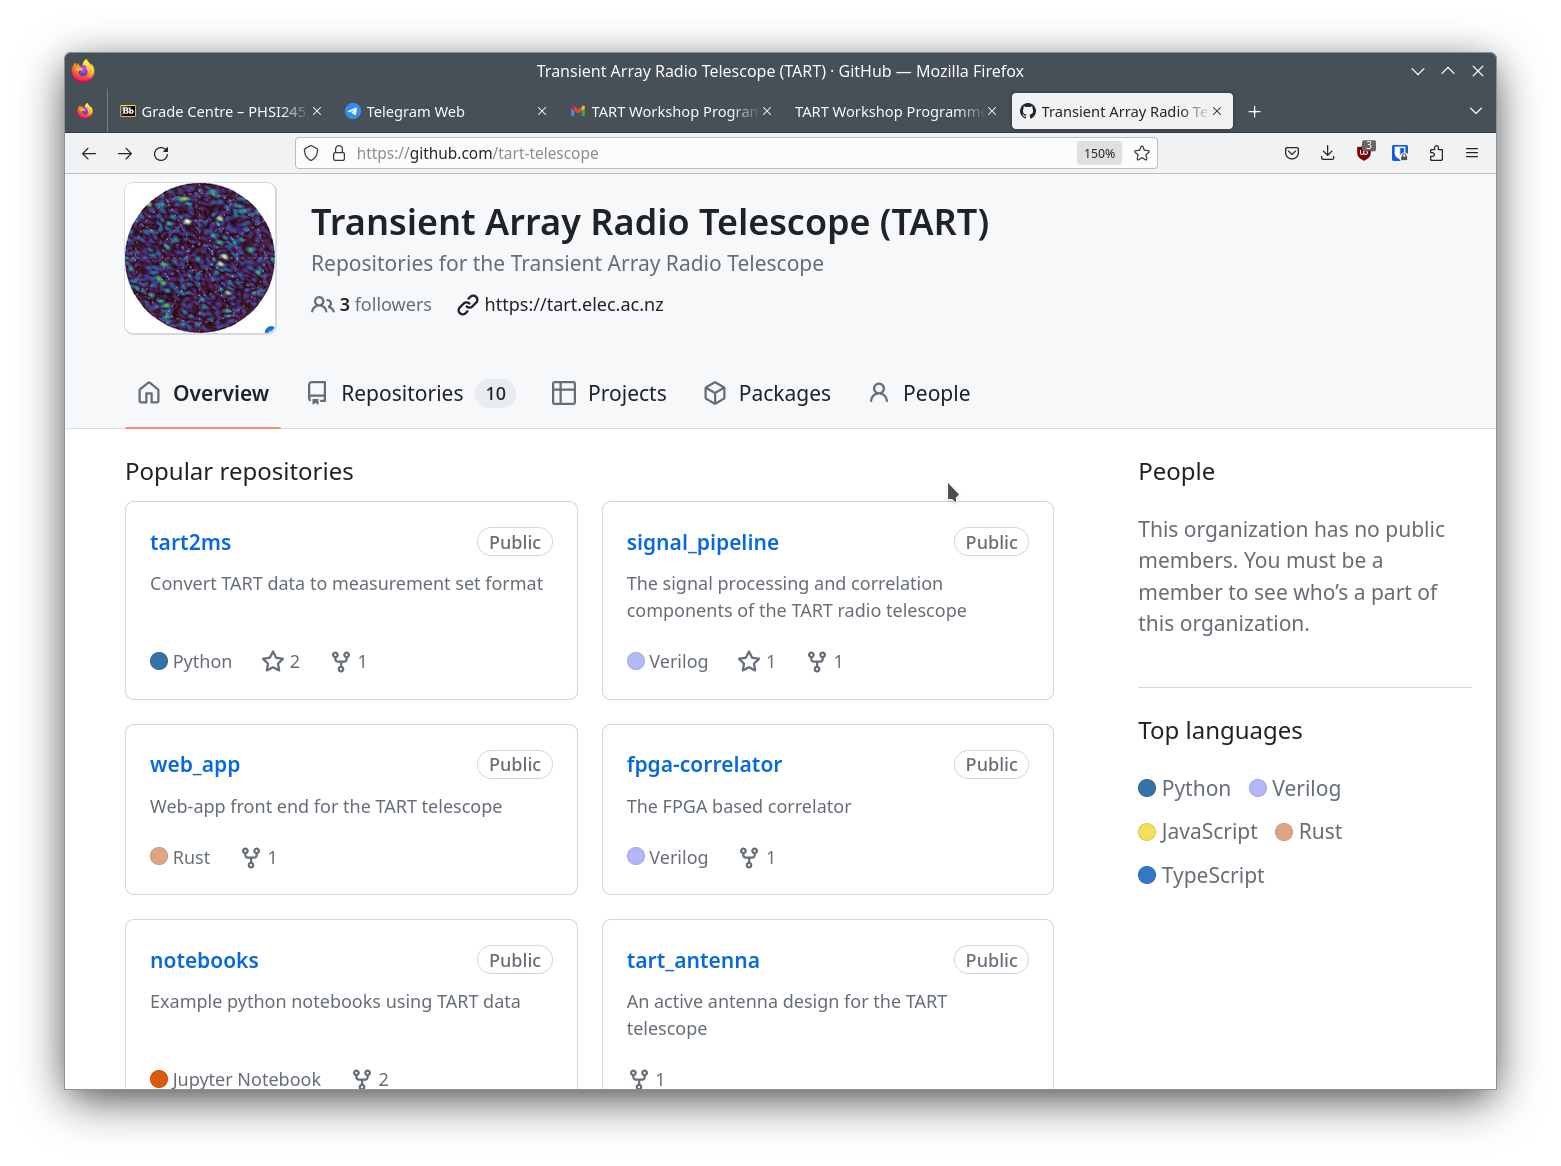
\includegraphics[width=\linewidth]{fig/screenshot_github.png}
  \end{column}
  \end{columns}
\end{frame}

 
\begin{frame}{TART components}
  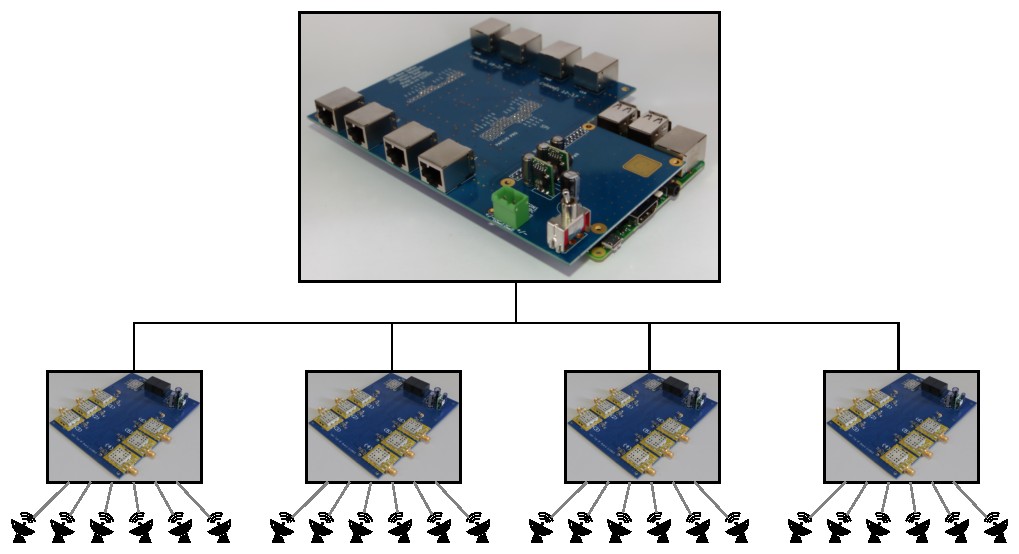
\includegraphics[width=\linewidth]{fig/tart_overview.pdf}
\end{frame}



\begin{frame}{GPS receiver chips}
 \begin{columns}
  \begin{column}{0.4\linewidth}
    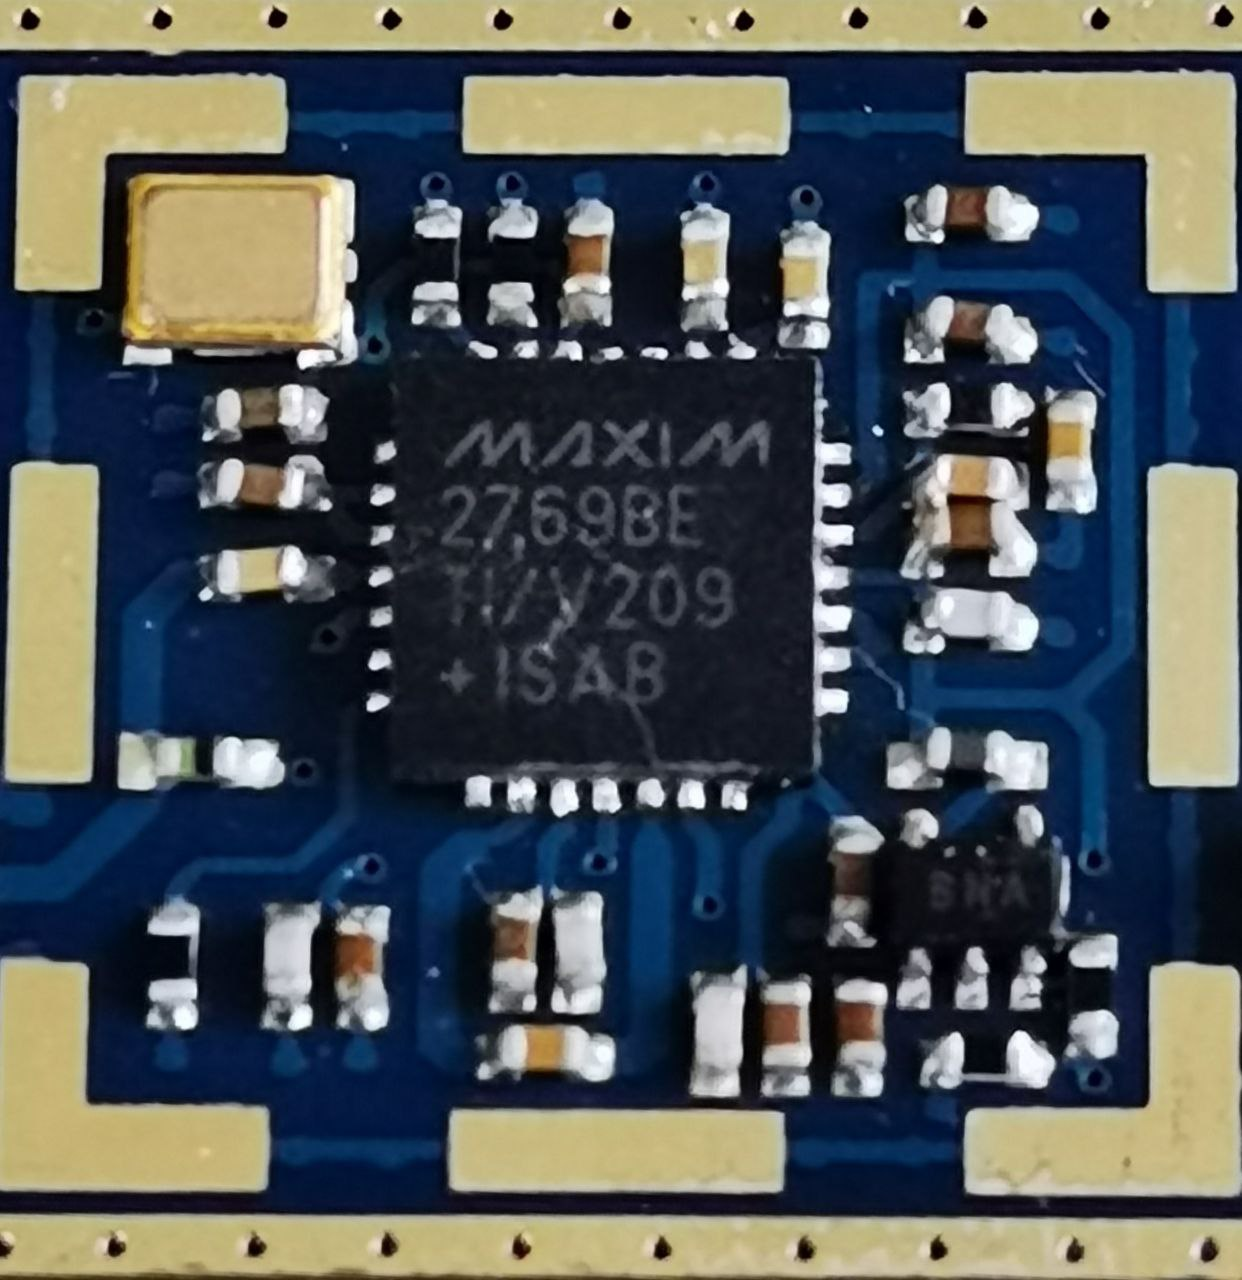
\includegraphics[width=\linewidth]{fig/max_2769.jpg}
  \end{column}
  \begin{column}{0.6\linewidth}
    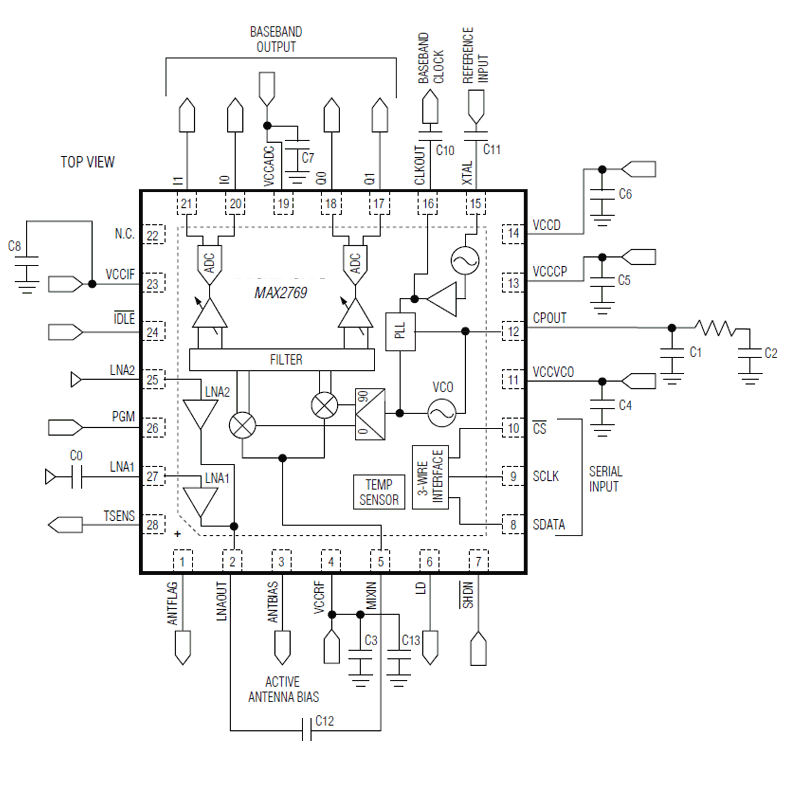
\includegraphics[width=\linewidth]{fig/max_2769_schem.png}
  \end{column}
  \end{columns}
\end{frame}

\begin{frame}{Upgrade Coming, late 2024}
  \begin{columns}
  \begin{column}{0.4\linewidth}
    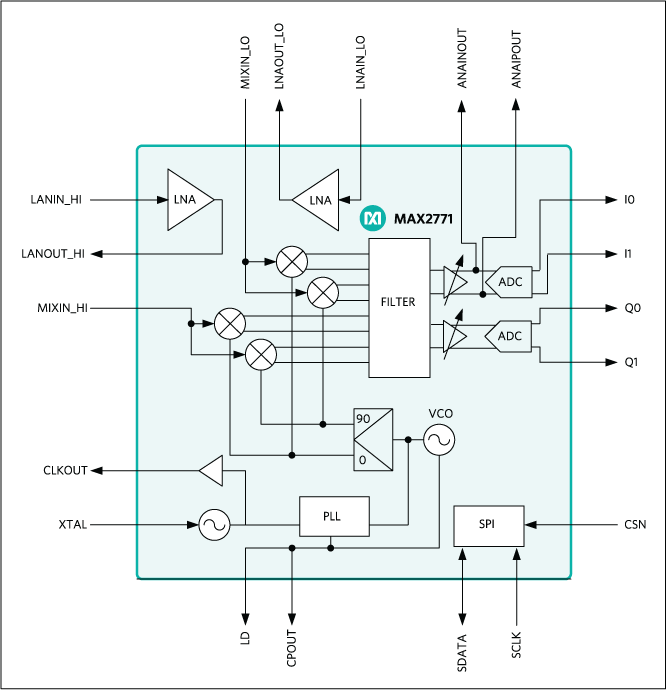
\includegraphics[width=\linewidth]{fig/max2771.png}
  \end{column}
  \begin{column}{0.6\linewidth}
  New Radio Front End.
\begin{itemize}
 \item 10x bandwidth (26 MHz)
 \item Zero IF operation
 \item 1160-1290 MHz and 1525-1610 MHz bands
 \item New radio module. TART-3
\end{itemize}

  \end{column}
  \end{columns}
\end{frame}

% \begin{frame}{Telescope Electronics}
% \centering
%  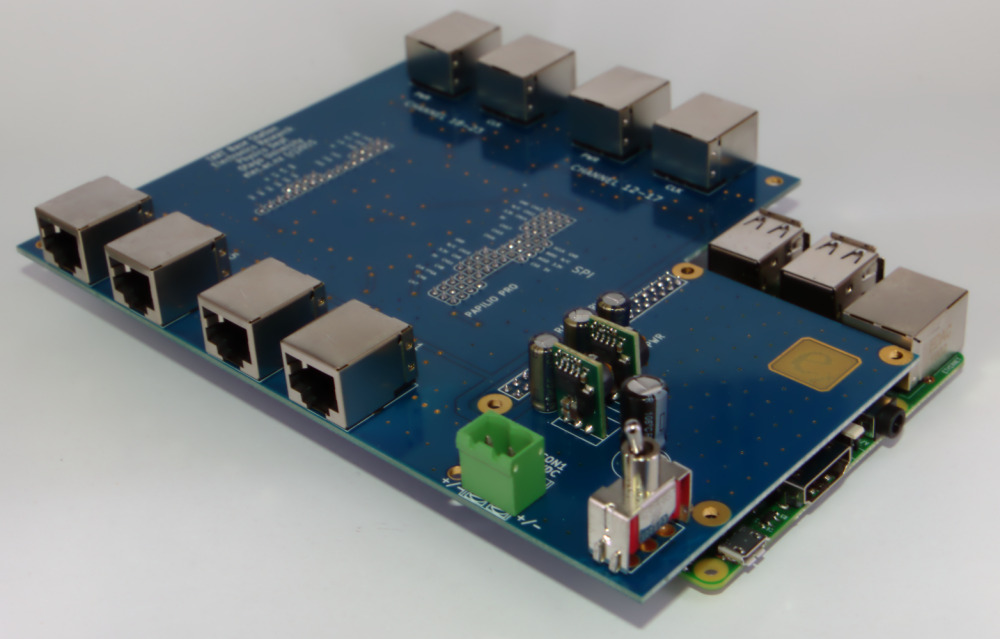
\includegraphics[height=0.4\textheight]{fig/control_board_photo.jpg}
%  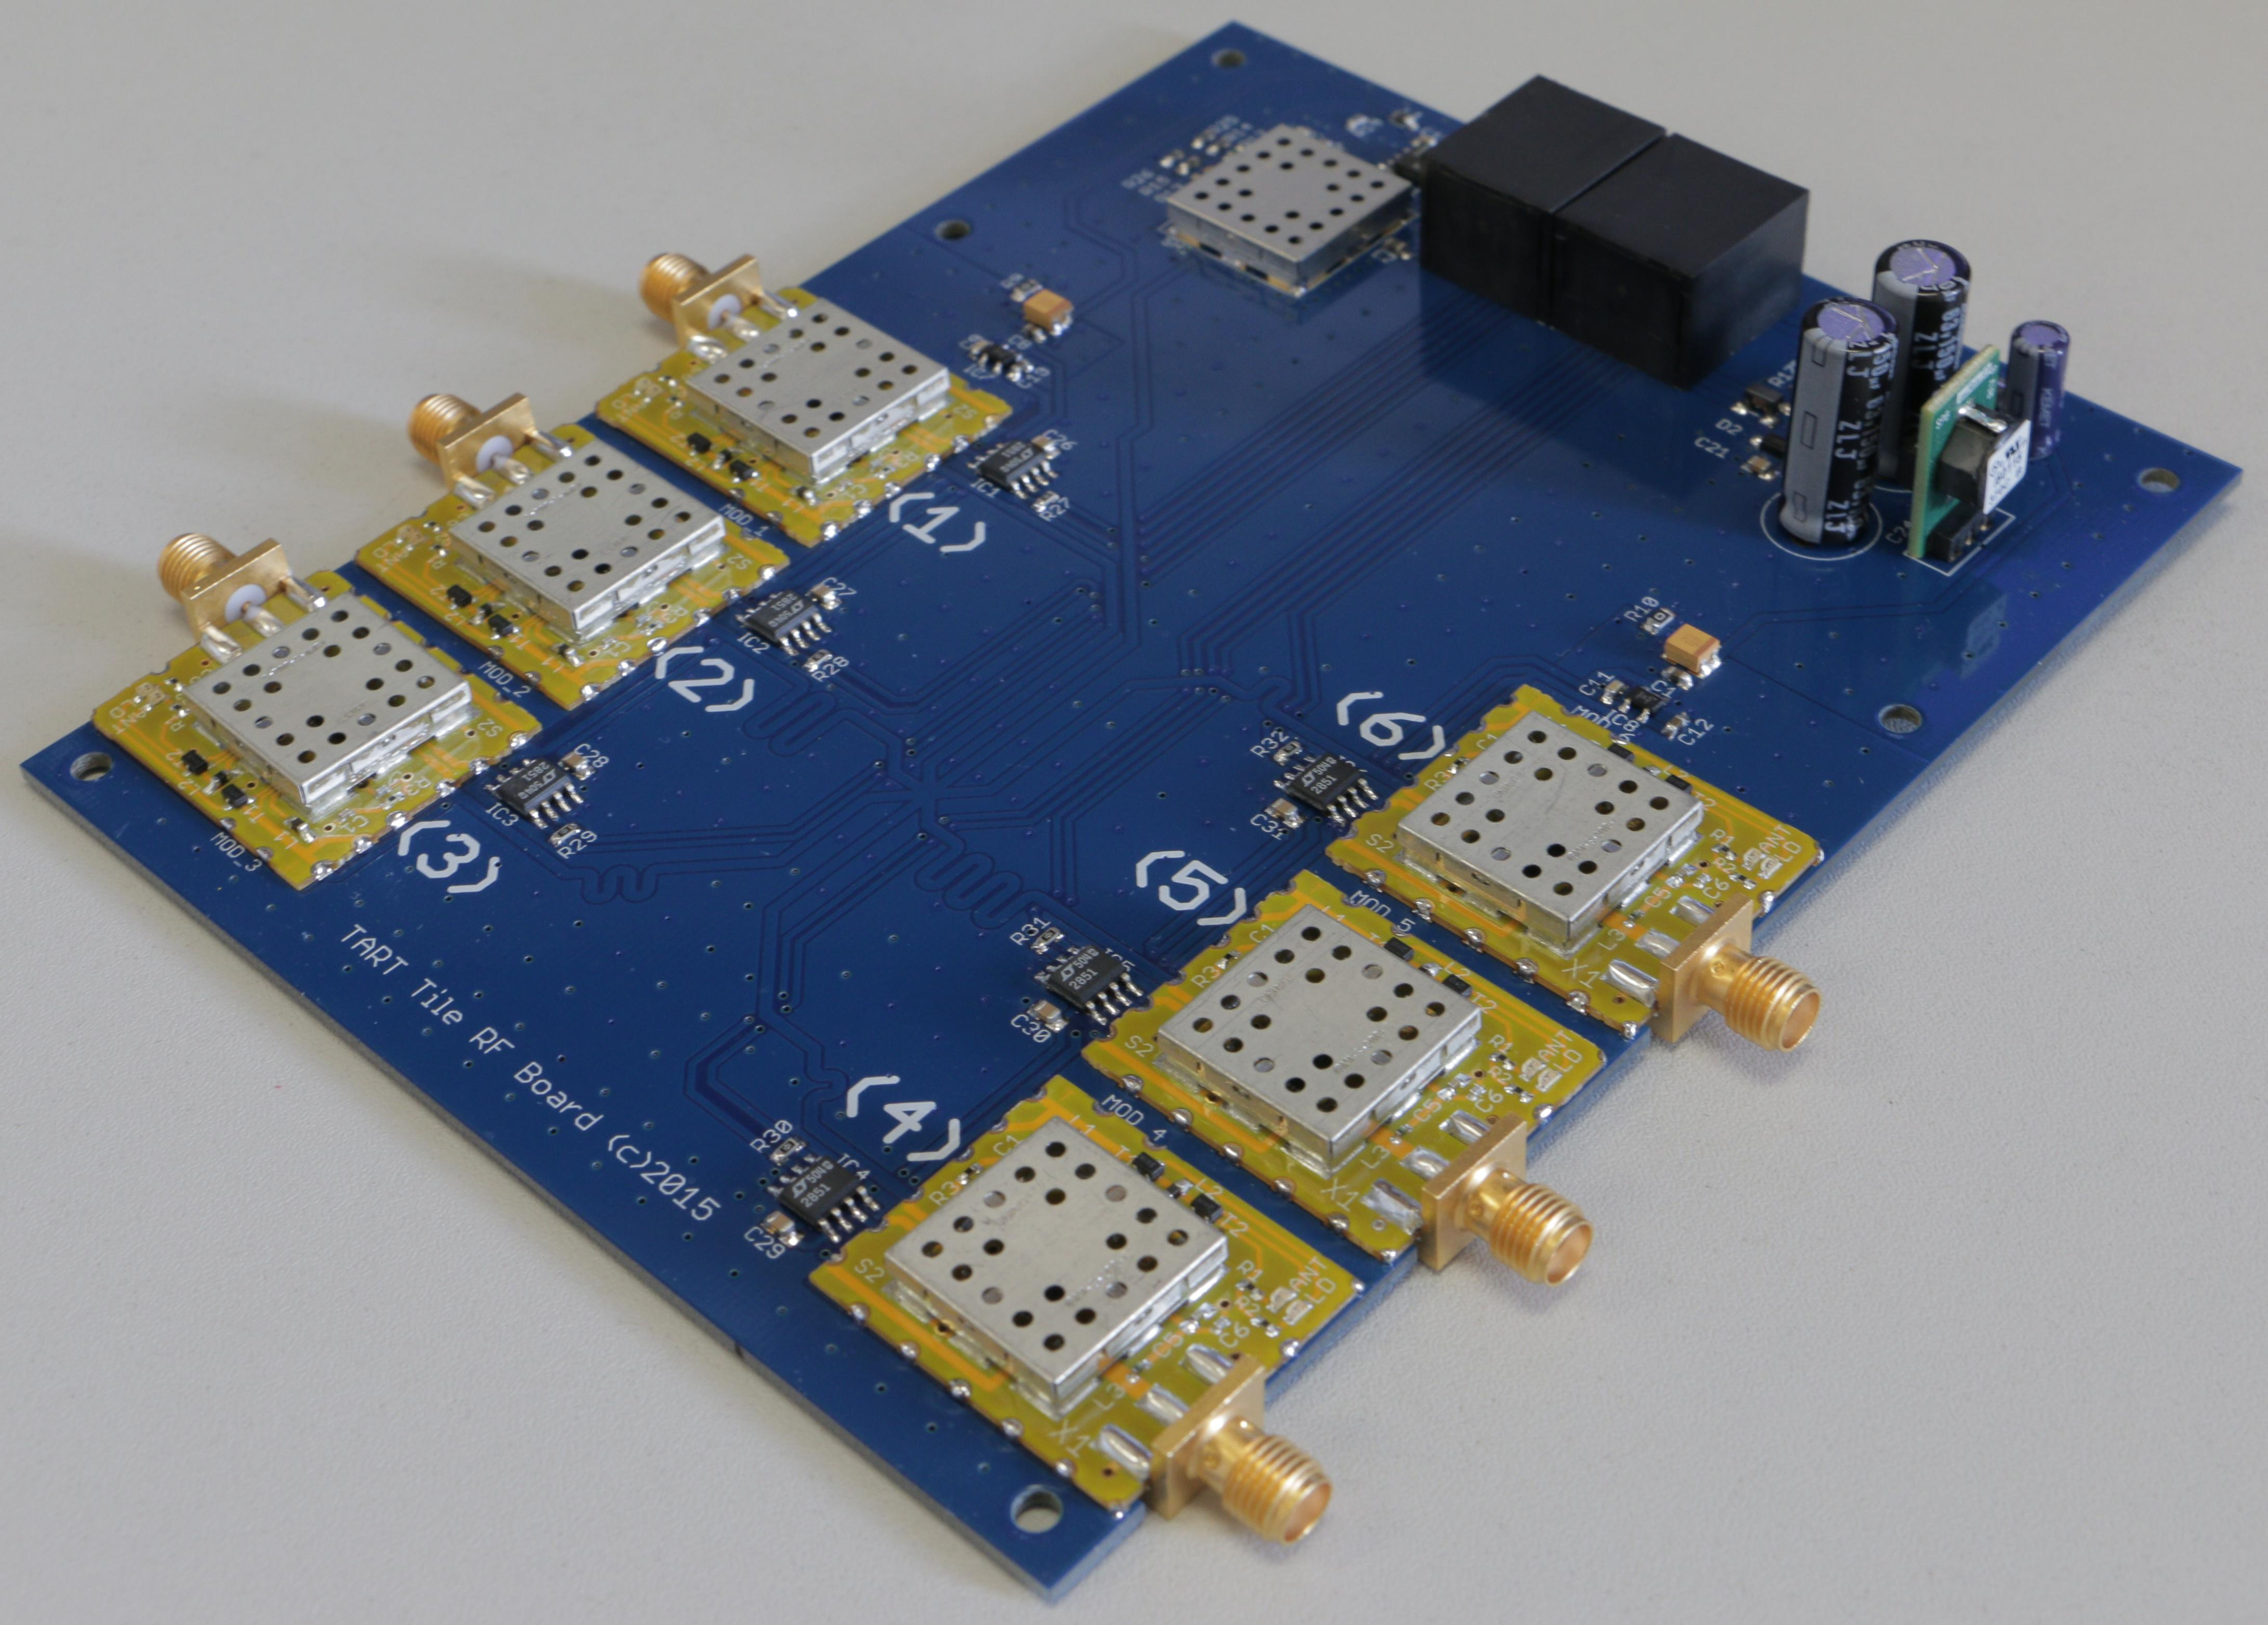
\includegraphics[height=0.4\textheight]{fig/radio_hub_photo.jpg}
% 
%  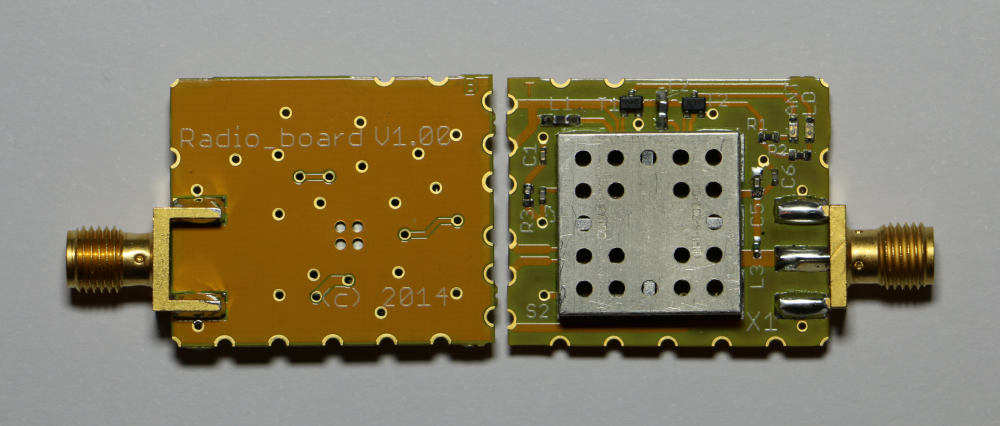
\includegraphics[width=0.7\linewidth]{fig/radio_module.png}
% \end{frame}
% 


\begin{frame}
 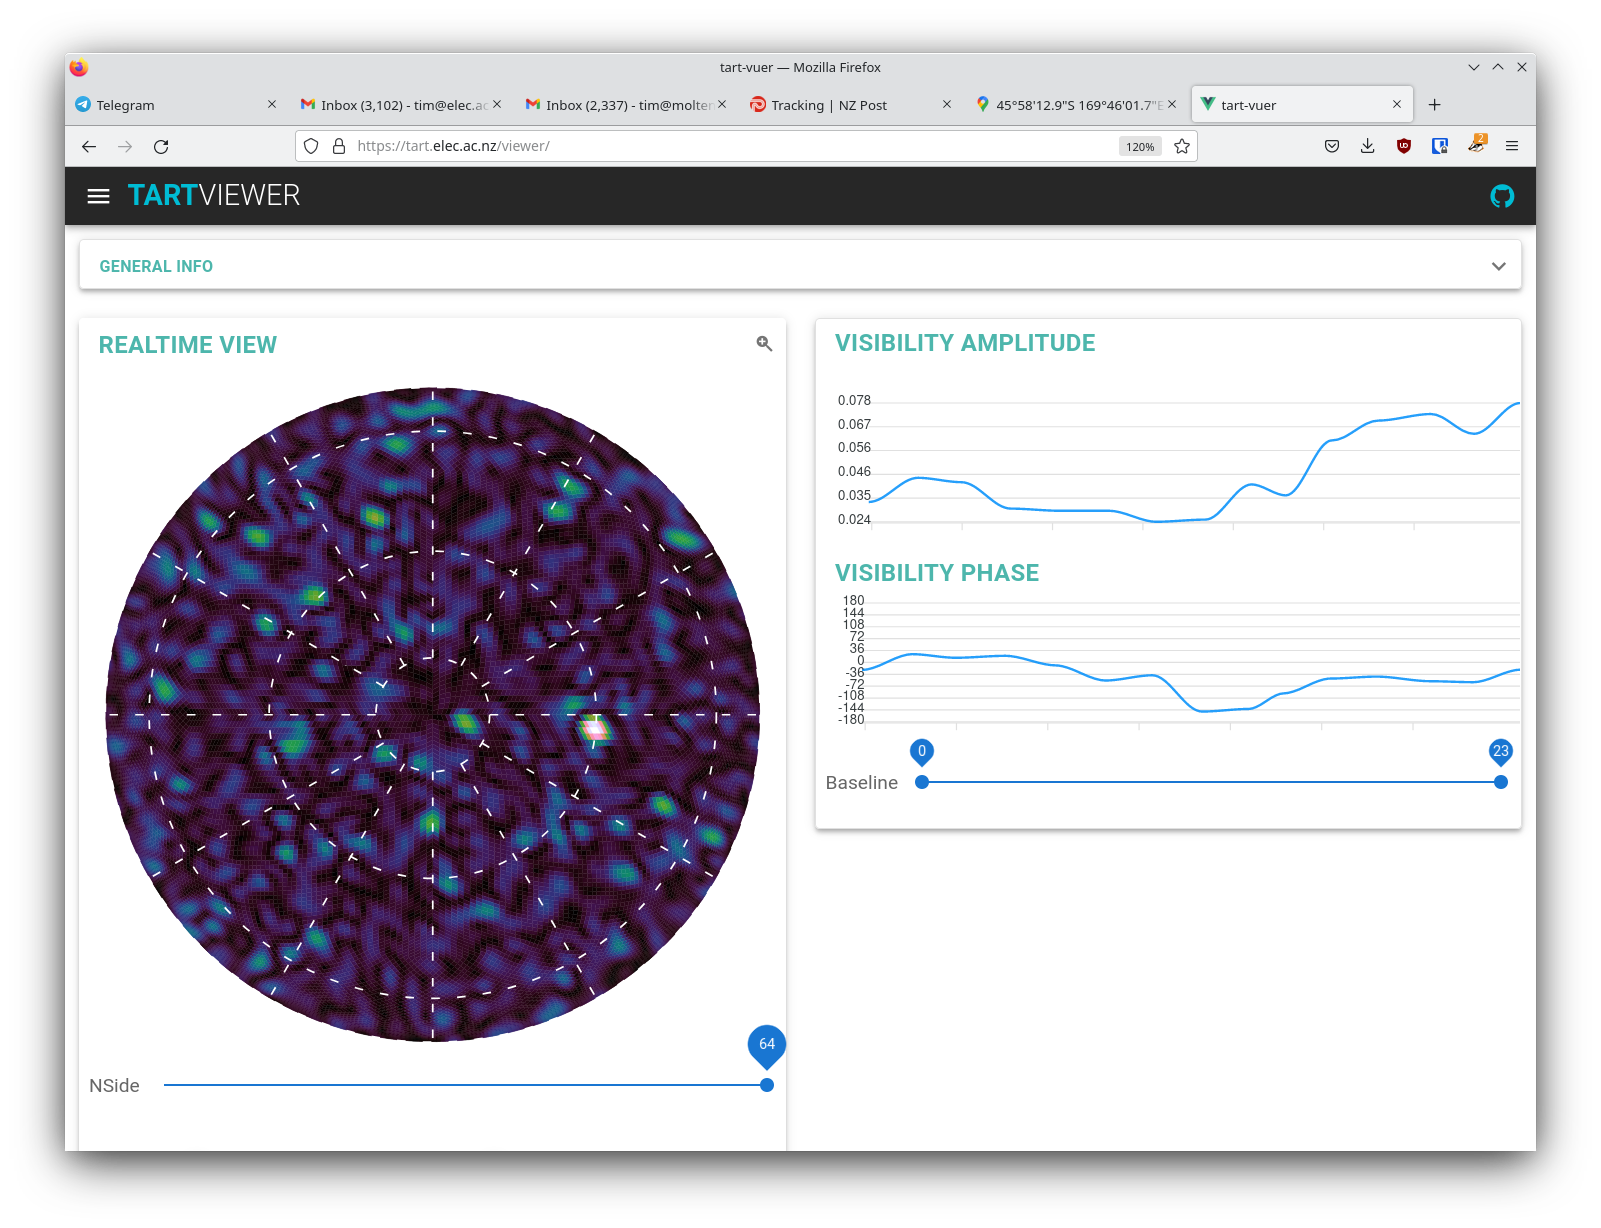
\includegraphics[width=\linewidth]{fig/browser_view.png}
\end{frame}

\begin{frame}{Synthesis Imaging}
Measure complex visibility $V_{ij}$ by correlating signals from antenna $i$ and $j$.
\[ V_{ij} = \frac{1}{T} \int_0^T E_i(t) E_j^{\star}(t) dt \]
\begin{columns}
 \begin{column}{0.55\linewidth}
\begin{enumerate}
 \item 276 Pairs of antennas
 \item 16.368 MHz sampling rate per antenna
 \item Real-time correlation in FPGA
 \item 4.5 Giga MAC per second
 \item T $\sim$ 1 second
\end{enumerate}
 \end{column}
 \begin{column}{0.45\linewidth}
 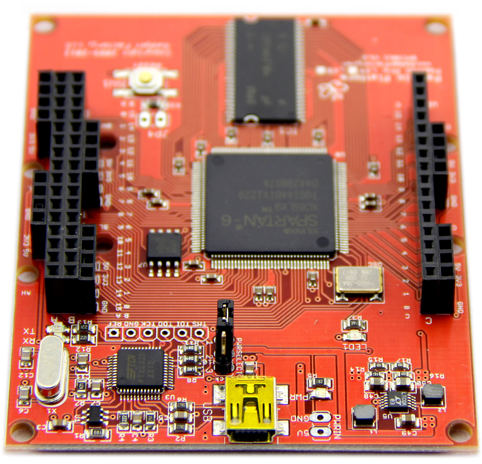
\includegraphics[width=\linewidth]{fig/papilio_pro.jpg}
 \end{column}
\end{columns}

\end{frame}

\begin{frame}{Synthesis Continued...}
Fourier transform relationship between radio sky brightness $I(l,m)$ and
visibility $V(u,v)$,
\[
  V(u,v) = \int I(l,m) e^{2\pi j(lu  + mv)} dl dm
\]
Obtain $I(l,m)$ through inverse Fourier transform of $V(u,v)$, 
\[
 I(l,m) = \mathscr{F}^{-1}\{V(u,v)\}
\]
where $V(u,v)$ is the visibility function sampled in the $uv$-plane at the locations of each antenna $(u_{ij},v_{ij})$ pair. 
\end{frame}


\begin{frame}{Tart Imaging Results}
\begin{center}
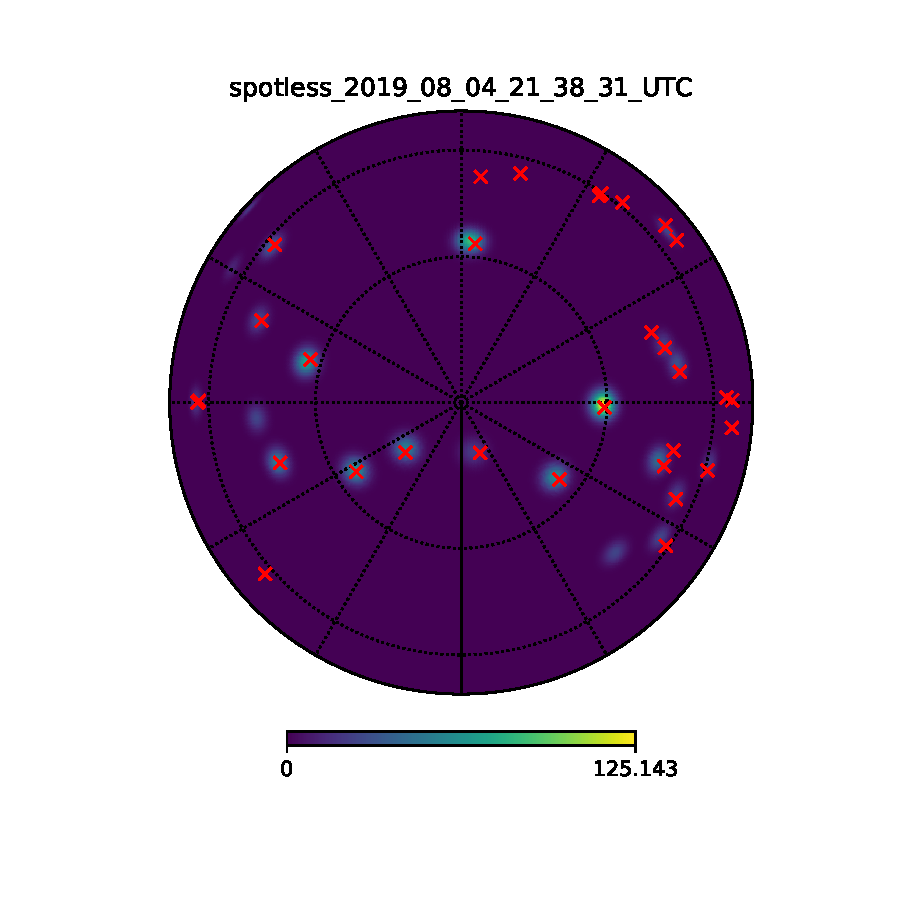
\includegraphics[width=0.6\linewidth]{fig/tart_snapshot.pdf}\\
 \hyperlinkmovie{A Video}{https://tart.elec.ac.nz/old/strange{\_}flyby.webm}
 \end{center}
\end{frame}

\begin{frame}{UFO}
\begin{center}
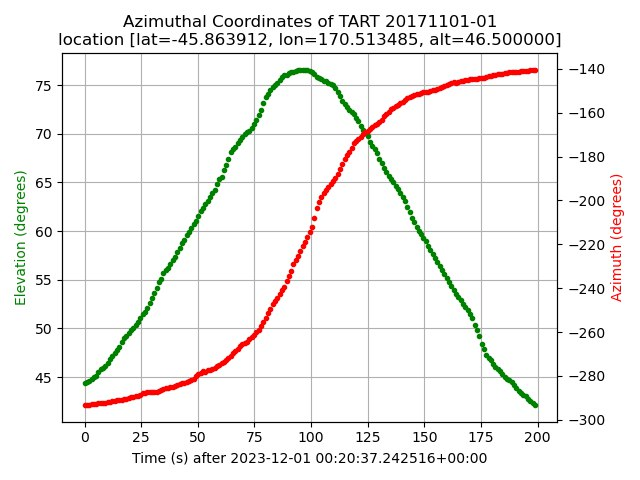
\includegraphics[width=0.8\linewidth]{fig/elaz.jpg}\\
 Consistent with something in low-earth orbit.
 \end{center}
\end{frame}

% 
% 
% \begin{frame}{The Dirty Image}
% For the TART telescope there are 24 antennas, 
% and 522 antenna pairs
% \begin{columns}
%  \begin{column}{0.5\textwidth}
%  \begin{figure}
% \includegraphics[width=\linewidth]{../../papers/2019_iceaa/uv_plane_init.pdf}
% \caption{U-V antenna pairs}
%  \end{figure}
%  \end{column}
%  \begin{column}{0.5\textwidth}
%  \begin{figure}
%  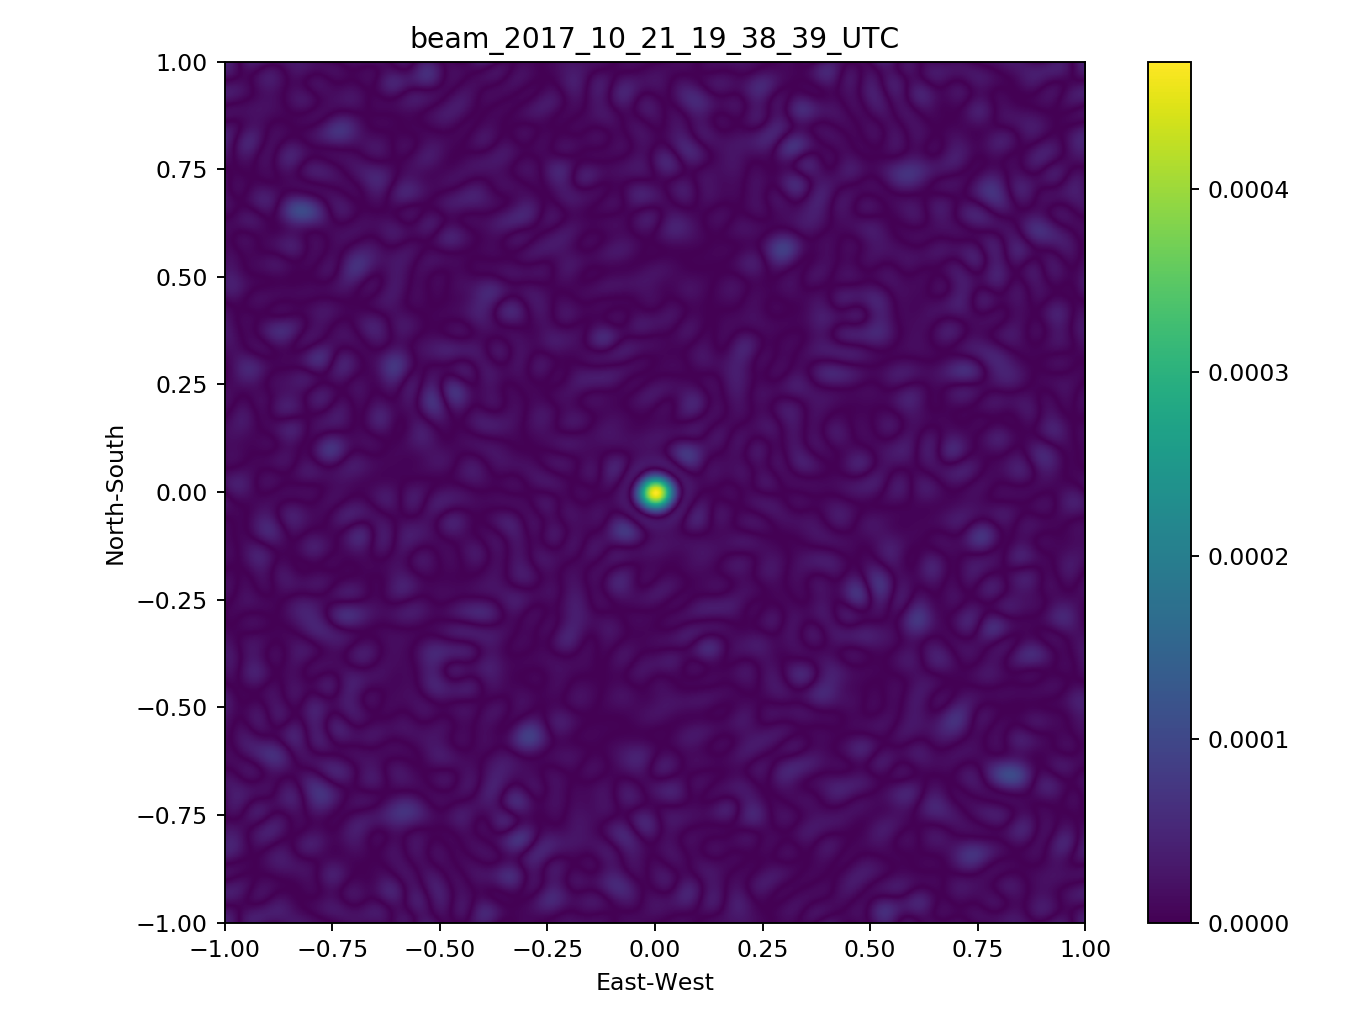
\includegraphics[width=\linewidth]{fig/beam_2017_10_21_19_38_39_UTC.png}
% % \includegraphics[width=\linewidth]{/home/tim/github/projects/max/phd/talk/nzip/pdf/dirty_beam_power_init.pdf}  
% \caption{Inverse Fourier Transform}
%  \end{figure}
%  \end{column}
% \end{columns}
% 
% \end{frame}
% % 
% % 
% % \begin{frame}{Swithing it on: Uncalibrated Image}
% % \begin{figure}
% % \includegraphics[height=0.9\textheight]{../../papers/2019_iceaa/uncalibrated_image.png} 
% % \end{figure}
% % \end{frame}
% % 
% % 
% % % \begin{frame}{CLEAN: H\"ogbom 1974}
% % % \begin{columns}
% % %  \begin{column}{0.5\linewidth}
% % % %  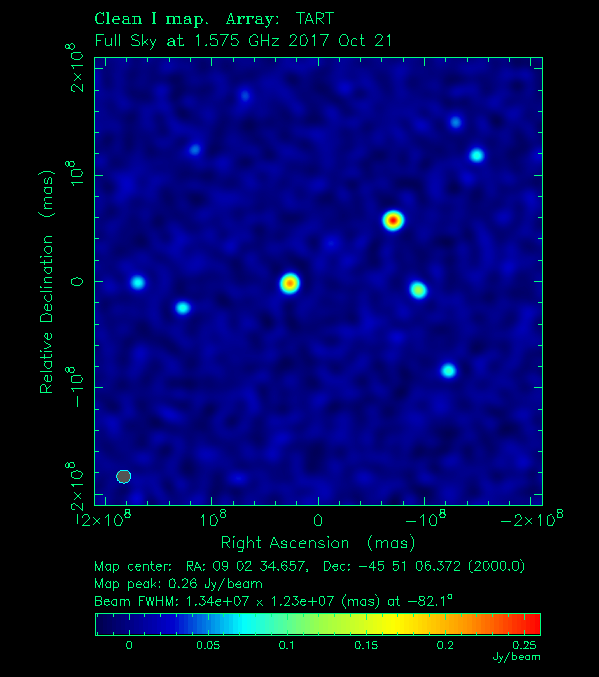
\includegraphics[width=\linewidth]{2017_10_21_19_38_39_UTC_uvfits_difmap.png}
% % %   \end{column}
% % %  \begin{column}{0.5\linewidth}
% % %   Image is the sum of point sources and a residual
% % %   \begin{eqnarray*}
% % %  I(l,m) & = & A_0 \delta(l_0, m_0) + I_0(l,m) \\
% % %  I_0(l,m)  & = & A_1 \delta(l_1, m_1) + I_1(l,m) \\
% % % 	   & = & \ldots
% % %   \end{eqnarray*}
% % %  \end{column}
% % % \end{columns}
% % % \end{frame}
% % 
% % \subsection{Satellites as Guide Stars}
% % 
% % \begin{frame}{The Guide Stars}
% %  \begin{columns}
% %   \begin{column}{0.5\linewidth}
% %    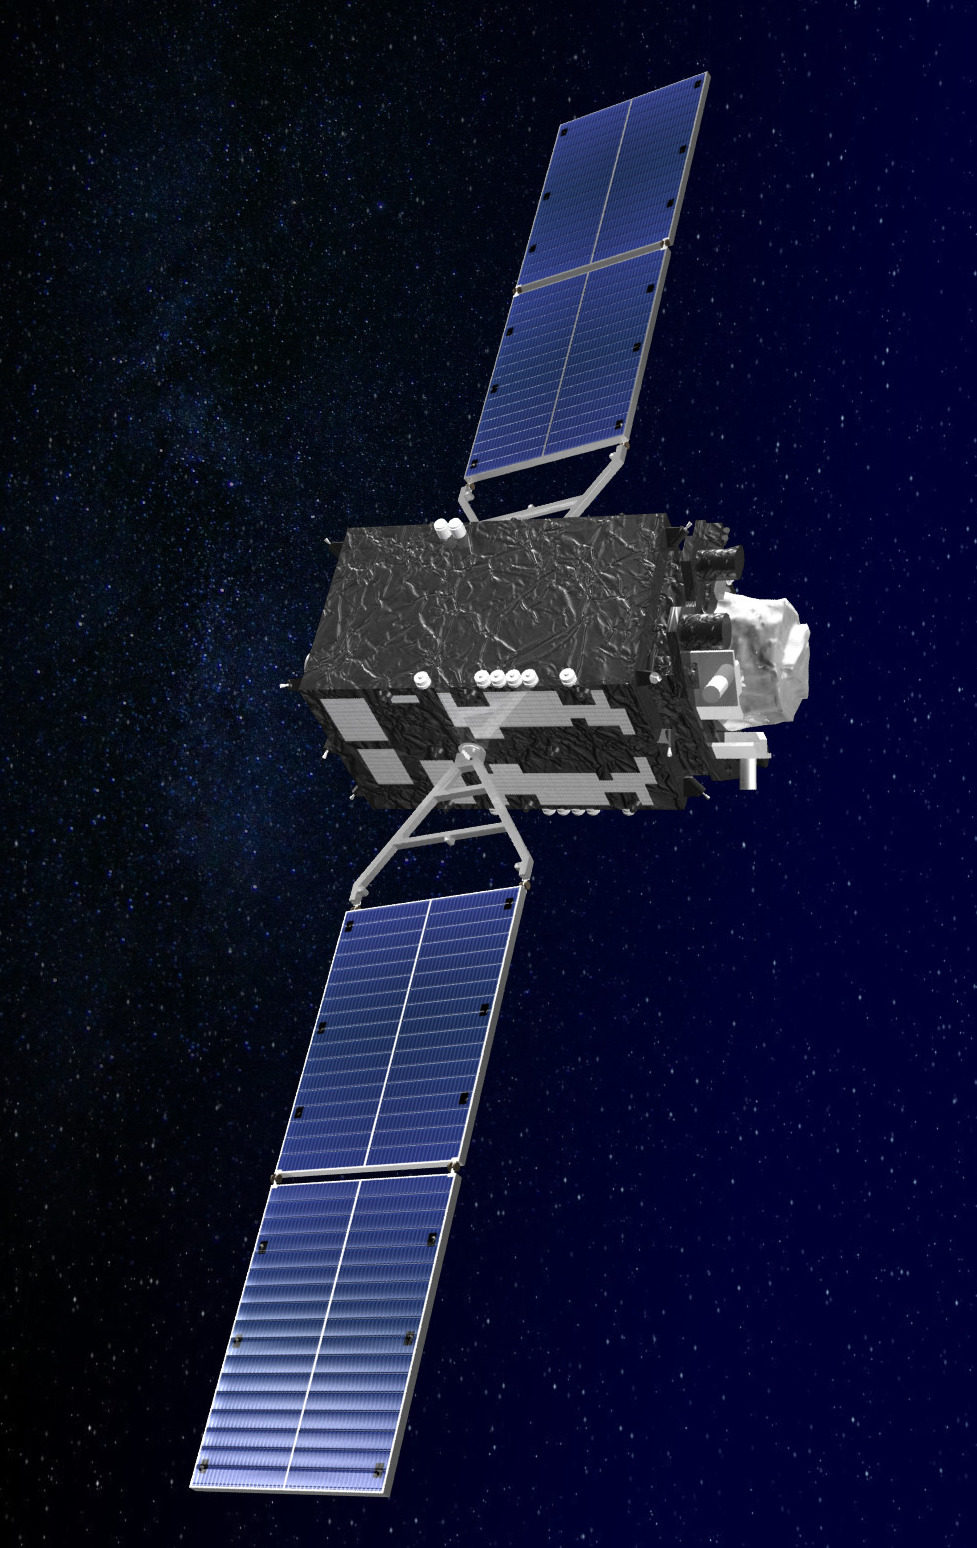
\includegraphics[height=0.9\textheight]{../sarao_bursary_2019/fig/QZS-1.jpg}
% %   \end{column}
% %   \begin{column}{0.5\linewidth}
% %   \begin{itemize}
% %    \item Position known to millimeters
% %    \item $>20000$ km away (point sources)
% %    \item Signal is `noise-like'
% %   \end{itemize}
% %    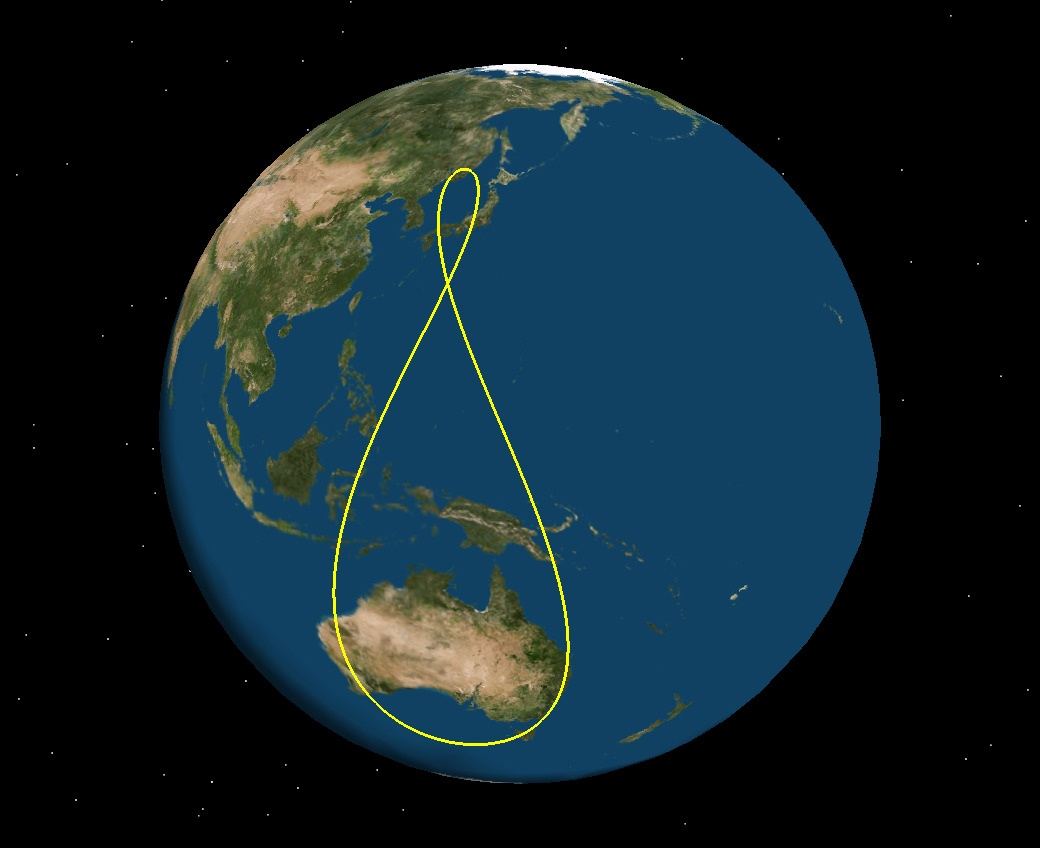
\includegraphics[width=\textwidth]{fig/qzss_ground_track.jpg}
% %    {\tiny Image: JAXA}
% %   \end{column}
% %  \end{columns}
% % \end{frame}
% % 
% 
% 
% \begin{frame}{Calibrated Clean Image}
% \begin{center}
% \includegraphics[height=0.9\textheight]{{../../papers/2019_iceaa/tart_clean.png}}
% \end{center}
% \end{frame}

\section{Building the TART Community}

\frame{\tableofcontents[currentsection]}

\begin{frame}{Workshops: Building the TART Community}
 \begin{columns}
  \begin{column}{0.5\linewidth}
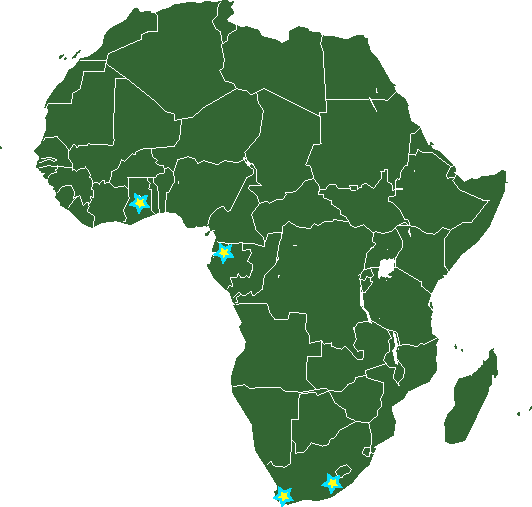
\includegraphics[width=\linewidth]{fig/Africa.pdf}
  \end{column}
  \begin{column}{0.5\linewidth}
  \begin{itemize}
   \item Week-long workshops
   \item Mornings: Lectures on radio astronomy
   \item Afternoons: Building a TART
   \item Joint supervision between members,
  \end{itemize}
  \vspace{1cm}
   
\includegraphics[width=\linewidth]{fig/workshop-partners.png}
\end{column}
 \end{columns}
\end{frame}

\begin{frame}{What the future holds}
    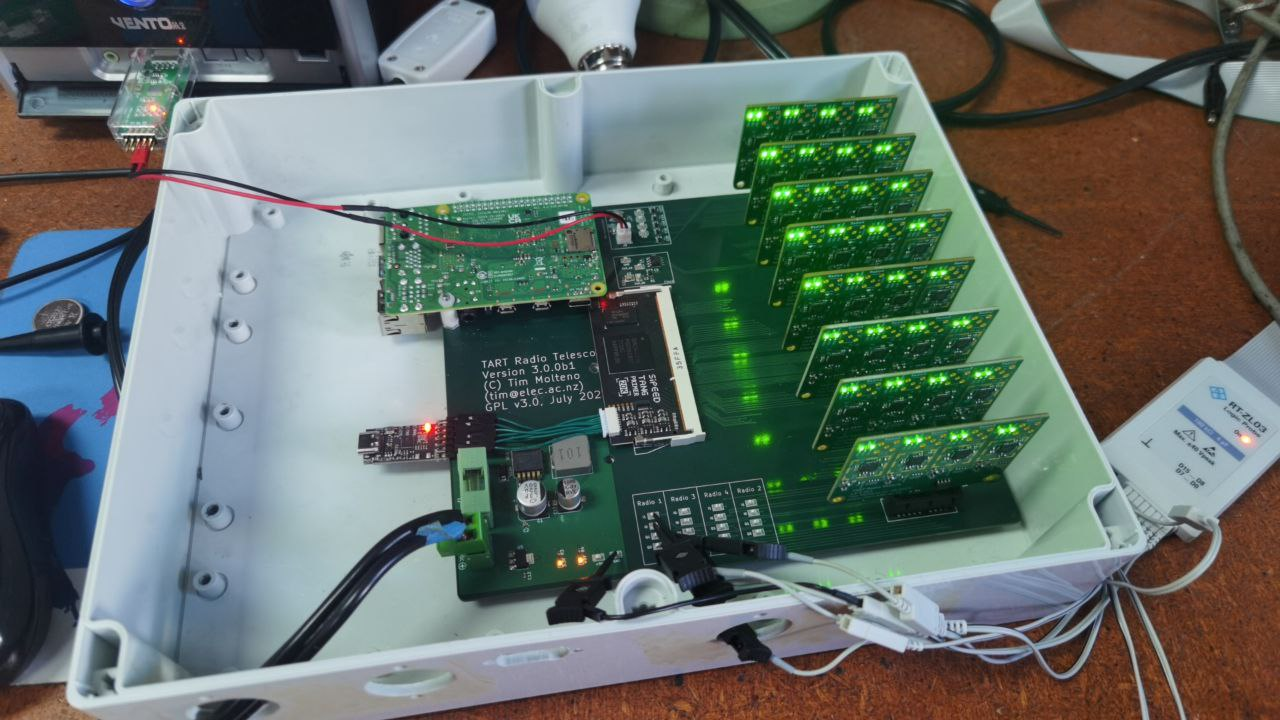
\includegraphics[width=\linewidth]{fig/tart3.jpg}
\end{frame}
\begin{frame}{TART-3}
 \begin{columns}
  \begin{column}{0.6\linewidth}
    \begin{itemize}
    \item TART 3.0. 32-Antennas, modular
    \item Transient event detection
    \item More workshops!
    \item Automatic tracking of space Debris
    \item New imaging algorithms (Gridless, Direct from Data)
    \end{itemize}
  \end{column}
  \begin{column}{0.4\linewidth}
    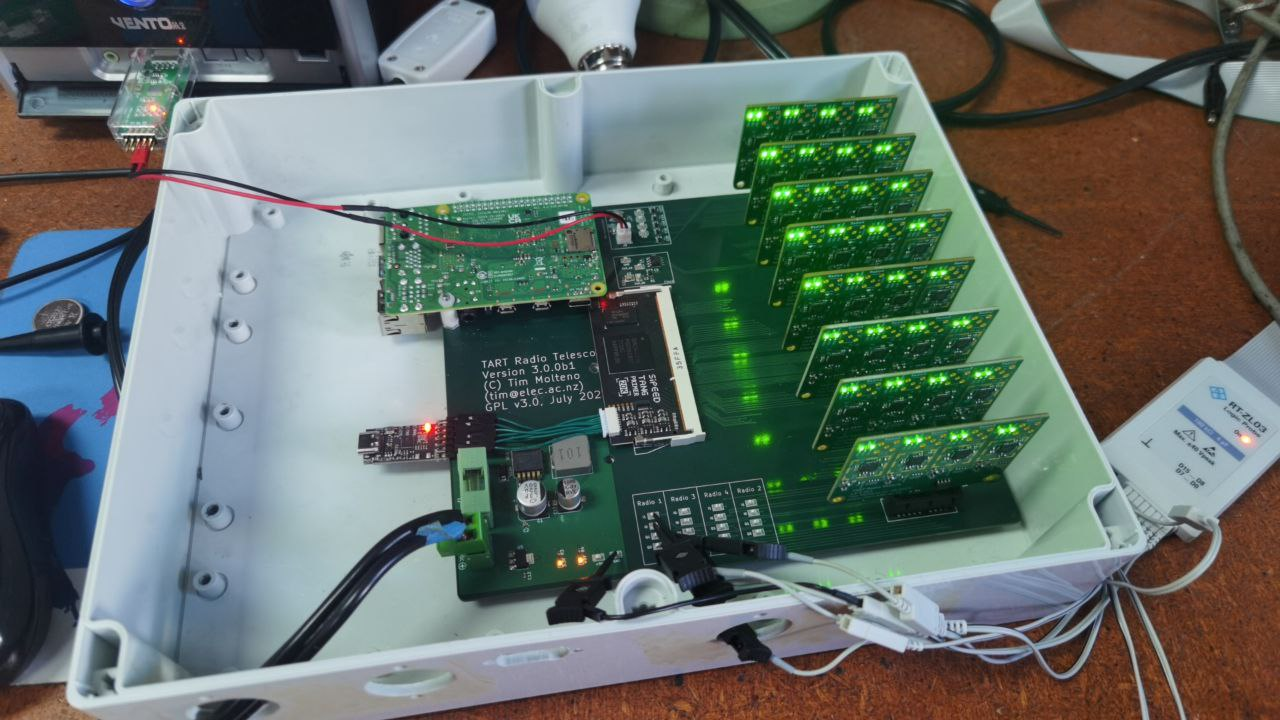
\includegraphics[width=\linewidth]{fig/tart3.jpg}
  \end{column}
\end{columns}
    \pause
    \begin{block}{}
     \begin{center} Questions? \end{center}
    \end{block}

\end{frame}


% \begin{frame}{Square Kilometer Array (www.skatelescope.org)}
% \includegraphics[width=\linewidth]{fig/1920px-SKA_overview.jpg}
% \end{frame}


\end{document}
